%% Text body begins.
%%
\section{Introduction}
\label{sec:introduction}

%% Leave page number of the first page empty
%% 
\thispagestyle{empty}

Modern enterprise-grade AI systems face continuously increasing resource constraints, in addition to growing operational expenditures driven by a rapid acceleration in corporate AI integration and exponential growth in the demand for AI computing capacity \citep{StanfordAIIndex2026}. Although API providers frequently lower unit token pricing, overall costs continue to rise due to explosive token usage and the complexity of multi-step agentic workflows that use the latest foundational large language models (LLMs) \citep{chen2024frugalgpt, GoogleVertexAIPricing}. This highlights the critical need for optimization across all phases of enterprise AI systems to ensure that computing resources are utilized as efficiently as possible.

This is especially true for Retrieval-Augmented Generation (RAG), which serves as a primary solution to mitigate critical limitations of modern LLMs, such as hallucination, the lack of up-to-date data, and the absence of domain-specific knowledge \citep{lewis2020rag, wu2025ragnlp}. By design, RAG inherently increases token consumption, particularly input tokens, as the core concept relies on prepending retrieved document context to user queries to generate more grounded responses. Within the retrieval module, a central challenge lies in finding the optimal balance between retrieval efficiency and the quality of the retrieved information \citep{wu2025ragnlp}. While various optimization strategies have been proposed in contemporary literature \citep{wu2025ragnlp, zhao2024ragandbeyond}, they are typically evaluated on static benchmarks and lack direct integration with industry-standard, production-grade languages and frameworks such as Java and Spring AI \citep{springai}.

The primary objective of this thesis is to investigate state-of-the-art optimization strategies for RAG systems, and the main contribution is to evaluate how these strategies perform within enterprise environments. Furthermore, this work demonstrates how these optimization strategies can be systematically evaluated and integrated within an enterprise Java and Spring AI infrastructure. To establish a focused scope, four specific optimization strategies are analyzed in detail: model cascading \citep{chen2024frugalgpt}, small-to-big retrieval \citep{lumer2026rethinking}, semantic re-ranking \citep{yu2024rankrag}, and prompt caching \citep{gim2024promptcache}. 

Each of these methods addresses a distinct phase of the RAG pipeline. Model cascading and small-to-big retrieval optimize the query and retrieval stages, whereas semantic re-ranking refines the retrieved results to minimize prompt size and maximize contextual relevance. Prompt caching, on the other hand, stores the precomputed key-value (KV) attention states of static prompt prefixes in memory, thereby accelerating the generator's prefill phase and reducing input token costs.

Many of these optimization strategies are typically evaluated in isolation, leaving a gap in the literature regarding how they interact when combined. For example, expanding context windows via small-to-big retrieval increases the proportion of dynamic, uncached tokens relative to the static cached prefix, potentially diluting the relative latency and cost savings of prompt caching. In addition, while model cascading may increase \textit{per-query} latency for complex tasks routed to more capable models, it decreases \textit{average} latency overall by resolving simpler tasks with faster, less capable models.

Evaluating and resolving these interactive conflicts is crucial for high-volume enterprise applications, such as customer support systems, where operational requirements are exceptionally rigorous. In these environments, minor delays and incremental token usage quickly compound into systemic instability, elevated latencies, and escalating operational costs. Furthermore, hallucinated or erroneous outputs present substantial risks of reputational damage and potential financial liabilities \citep{aba2024aircanada}. Because enterprise systems must strictly navigate these critical constraints, cost, latency, and output quality are established as the primary evaluation metrics for this thesis. To guide this investigation, this study addresses the four primary research questions summarized in Table~\ref{tab:research_questions}.

\begin{table}[htbp]
    \centering
    \caption[Primary research questions]{Primary research questions addressed in this thesis.}
    \label{tab:research_questions}
    \begin{tabularx}{\textwidth}{l X}
    \toprule
    \textbf{} & \textbf{Research Question} \\
    \midrule
    \textbf{RQ1} & \textbf{Latency:} How do small-to-big retrieval, semantic re-ranking, prompt caching, and model
  cascading affect the latency profile (specifically Time to First Token [TTFT] and overall end-to-end execution
  latency) of a RAG system? \\
    \addlinespace
    \textbf{RQ2} & \textbf{Cost:} To what extent do these optimization methods reduce the operational cost of the
  system, accounting for token pricing tiers, prompt caching discounts, and model cascading? \\
    \addlinespace
    \textbf{RQ3} & \textbf{Quality:} How do these optimizations impact retrieval and generation quality (measured by
  Context Precision, Context Recall, Faithfulness, and Answer Relevancy) compared to a naive RAG baseline? \\
    \addlinespace
    \textbf{RQ4} & \textbf{Interaction:} How do these optimization methods interact when combined, and what is the
  optimal equilibrium between latency, cost, and quality in an enterprise customer support system? \\
    \bottomrule
    \end{tabularx}
\end{table}

The rest of the thesis is structured as follows: Chapter~\ref{sec:technical_bg} provides the technical background on large language models and naive retrieval-augmented generation architectures, while Chapter~\ref{sec:literature-review} examines the current literature on modular RAG optimization methods. Research methods are introduced in Chapter~\ref{sec:methods}, and the empirical results are presented in Chapter~\ref{sec:results}. Finally, the findings and systemic trade-offs are discussed in Chapter~\ref{sec:discussion}, and concluding remarks are provided in Chapter~\ref{sec:conclusion}.


\clearpage

\section{Technical background}

Retrieval-Augmented Generation (RAG) offers an architectural solution to mitigate several of the most fundamental limitations of Large Language Models (LLMs), such as hallucination, the lack of up-to-date data, and the lack of domain-specific knowledge \cite{wu2024ragnlp}. To establish a comprehensive understanding of these concepts, this chapter provides the necessary technical background for both technologies. The first section examines the architectural foundations and inherent drawbacks of LLMs\footnote{This section is partly based on the author's bachelor's thesis \cite{asunmaa2025large}.}, while the subsequent section focuses on the core principles and operational mechanics of plain vanilla RAG.

\label{sec:technical_bg}
Retrieval-Augmented Generation (RAG) offers an architectural solution to mitigate several of the most fundamental limitations of Large Language Models (LLMs), such as hallucination, the lack of up-to-date data, and the lack of domain-specific knowledge \cite{wu2025ragnlp}. To establish a comprehensive understanding of these concepts, this chapter provides the necessary technical background for both technologies. The first section examines the architectural foundations and inherent drawbacks of LLMs\footnote{This section is partly based on the author's bachelor's thesis \cite{asunmaa2025large}.}, while the subsequent section focuses on the core principles and operational mechanics of plain vanilla RAG.

\subsection{Large-Language Models}
\label{chapter:LLM}

\subsubsection{Evolution and Adoption of Language Models}
Natural language processing (NLP) has traditionally focused on enabling computer systems to understand human-generated language and acquire knowledge \cite{RussellNorvig2010}. Early statistical approaches, such as n-gram language models, attempted to resolve the inherent ambiguity of natural language by predicting the probability distribution of word sequences \cite{RussellNorvig2010}. While these traditional models could perform structured tasks like rule-based information extraction or spam filtering, their capability to comprehend semantic nuances and manage complex linguistic tasks remained limited \cite{LLMSurvey}.

Many pre-trained language models (PLMs), such as GPT-2 \cite{radford2019language}, are based on the transformer architecture \cite{Vaswani2017}, which excels at handling long-range dependencies through parallel training. While early PLMs required task-specific fine-tuning to perform downstream applications \cite{bommasani2021opportunities}, modern large language models (LLMs) scale this architecture to hundreds of billions of parameters. According to \citet{LLMSurvey}, the transition from PLMs to LLMs is primarily characterized by this massive scale in parameters and training data, which gives rise to emergent abilities, enabling the models to solve complex tasks and follow instructions without explicit task-specific retraining.

Presently, large language models are among the most widely used technologies behind modern generative AI applications \citep{LLMSurvey}. Even though these models have demonstrated strong performance across various tasks, such as coding \citep{Coignion_2024}, and have been widely adopted\footnote{For instance, data aggregated in the report \cite{StanfordAIIndex2026} highlights a rapid acceleration in corporate AI integration. In Europe, corporate adoption in at least one business function was 91\% in 2025 compared to 57\% in 2023.}, they are not perfect. 

\subsubsection{Architectural and Operational Constraints}

Despite their capabilities, LLMs exhibit several major limitations, including biases, hallucinations, and the "Lost in the Middle" (LitM) phenomenon \citep{introgenai, liu2024lost}. Bias refers to the fact that the model’s output heavily depends on its training data, meaning that the generated content may include inappropriate language, conspiracy theories, or gender bias \citep{introgenai}. 

Due to the autoregressive nature of modern LLMs, these models are inherently prone to hallucinations, where they produce outputs that appear plausible but are factually incorrect \citep{ji2023survey}. This occurs because the models lack an intrinsic understanding of facts, but instead, they generate responses by predicting subsequent tokens based on statistical patterns learned during training. This relying mechanism draws entirely from the model's parametric knowledge, meaning the information is permanently embedded within the model's weights during the training phase \citep{bommasani2021opportunities}. This static nature, consequently, makes it computationally and environmentally expensive and impractical to frequently retrain or fine-tune entire models when the underlying information required to complete a task changes \cite{StanfordAIIndex2026}.

While the context windows, i.e., LLMs' input sizes, have grown significantly during the last couple of years, allowing models to process up to millions of input tokens \citep{geminiteam2024gemini, GoogleDeepMind2025Gemini3Flash}, these architectures consistently suffer from the LitM phenomenon. This problem refers to a limitation where models effectively utilize information located at the absolute beginning (primacy bias) or the end (recency bias) of the prompt, while failing to retrieve relevant facts buried within the middle sections \citep{liu2024lost}. In addition, utilizing massive contexts severely increases computational latency and operational expenses, as modern cloud LLM APIs employ token-based pricing models where input costs scale linearly with prompt length and often double when exceeding specific context thresholds \citep{GoogleVertexAIPricing}. These inherent limitations effectively prevent the full utilization of large context windows in production-grade enterprise environments when attempting to ingest massive enterprise knowledge bases directly into the prompt.

Another source of errors in the output is that the training data has a cutoff date, so it does not contain the most recent information and may generate incorrect answers to questions about recent events \citep{dhingra2022time}. To mitigate these limitations, modern LLM-based systems are integrated with web search capabilities to retrieve real-time information from the internet, a paradigm used, for example, by the Google Gemini model family \cite{geminiteam2024gemini}. While this integration helps keep responses up to date, it introduces an external dependency on the reliability of internet sources. Furthermore, relying purely on open-web search does not solve the challenge for enterprise environments, where the required knowledge is locked behind internal intranet pages and private corporate databases rather than publicly accessible web pages.

\subsection{Naive Retrieval-Augmented Generation}

To address the limitations detailed in the previous section, Retrieval-Augmented Generation (RAG) offers an architectural solution that decouples the LLM's reasoning capabilities from its static parametrized memory \citep{lewis2020rag}. RAG enriches the LLM's parametric knowledge with non-parametric data served dynamically from an external knowledge base. The LLM's output is based on the user's initial prompt, augmented with the data retrieved from the external knowledge base, and therefore forces the LLM to ground its response in the provided context rather than its parametrized data.

The retrieval-augmentation process requires both the source knowledge and the user query to be preprocessed. Preprocessing of the knowledge base contains three phases: chunking, vectorizing, and indexing. During this data preparation phase, source documents —such as PDF files— are chunked into smaller, more manageable segments\footnote{Early architectures like \citet{lewis2020rag} utilized fixed-length segments of 100 words, while modern architectures optimize segment lengths \citep{demourajunior2026adaptive}.}. These chunks are converted into numerical vectors using an embedding model so that their semantic meanings can be mathematically calculated, and they are subsequently stored in an indexed vector database \citep{gao2023retrieval}. During runtime inference, the user's initial prompt is vectorized using the same embedding model. The system then calculates the mathematical distance (e.g., cosine similarity) between the prompt vector and the stored vectors, retrieving the most relevant chunks from the database to augment the initial prompt \citep{johnson2019billion}.

The primary advantage of the RAG architecture lies in its reliance on an external knowledge base. When properly prompted, this mechanism significantly mitigates hallucinations by forcing the LLM to ground its output exclusively on the retrieved context \citep{shuster2021retrieval}. Furthermore, maintaining an external data repository is substantially more cost-effective and computationally practical than continuously retraining or fine-tuning the underlying model \citep{gao2023retrieval}, allowing enterprise systems to remain up-to-date in real time. From a data governance perspective, an external knowledge base ensures that sensitive corporate data remains secure and under internal control \cite{ni2025towards}. Lastly, by selectively retrieving only the most relevant documents, RAG compresses the required input context, thereby reducing API transaction costs and inference latency compared to naive long-context processing.

However, these benefits introduce distinct trade-offs. The major drawback of a naive RAG pipeline is the increased end-to-end latency of the system \citep{gao2023retrieval}. This latency overhead stems primarily from sequential network requests: first querying the embedding model and vector database, and subsequently transmitting the expanded prompt to the LLM. While modern vector distance calculations are highly optimized, the network overhead and the increased time-to-first-token (TTFT) caused by processing larger, augmented prompts add noticeable delay \citep{gao2023retrieval}. Consequently, if the RAG pipeline is not properly optimized, the final prompt can grow excessively large, rendering the production system both financially expensive and operationally slow.



\clearpage

\section{Literature review}
\label{sec:literature-review}
This chapter reviews the current literature on the four selected optimization techniques, focusing on the performance benefits each method provides in relation to the research questions. Relevant publications were identified on Google Scholar using keyword combinations of the optimization method and ``RAG'' or ``retrieval-augmented generation''. In addition, snowballing \cite{guidelines}, starting from comprehensive surveys (e.g., \cite{gan2025rag, gao2023retrieval, wu2024ragnlp}), was used to discover further relevant studies. Due to the rapid pace of development in this research area, the selected literature consists primarily of articles published after 2023. The remainder of this chapter is structured as follows: Section~\ref{lit:cascading} reviews model cascading and routing, Section~\ref{lit:retrieval} examines small-to-big retrieval, Section~\ref{lit:re_rank} covers semantic re-ranking, and Section~\ref{lit:caching} discusses prompt caching.
This chapter reviews the current literature on the four selected optimization techniques, focusing on the performance benefits each method provides in relation to the research questions. Relevant publications were identified on Google Scholar using keyword combinations of the optimization method and ``RAG'' or ``retrieval-augmented generation''. In addition, snowballing \cite{guidelines}, starting from comprehensive surveys (e.g., \cite{gan2025rag, gao2023retrieval, wu2025ragnlp}), was used to discover further relevant studies. Due to the rapid pace of development in this research area, the selected literature consists primarily of articles published after 2023. The remainder of this chapter is structured as follows: Section~\ref{lit:cascading} reviews model cascading and routing, Section~\ref{lit:retrieval} examines small-to-big retrieval, Section~\ref{lit:re_rank} covers semantic re-ranking, and Section~\ref{lit:caching} discusses prompt caching.

\subsection{Cascading}
\label{lit:cascading}
Modern RAG systems encounter diverse workloads, ranging from simple informational queries to highly complex analytical tasks. In production-grade enterprise environments — where high availability, low latency, and cost efficiency are critical constraints — a "one-size-fits-all" architecture is fundamentally sub-optimal \cite{jeong2024adaptive, chen2023frugalgpt}. It over-allocates expensive computational resources for trivial questions, yet may lack the retrieval depth and reasoning capacity required for complex queries. To mitigate this, model cascading or query routing can be employed to dynamically direct inputs to an appropriately scaled configuration of the RAG pipeline \cite{ong2025routellm}. For instance, a simple query can bypass the full pipeline and utilize a lightweight LLM with minimal context. Conversely, a complex query requiring synthesis across multiple enterprise knowledge bases can trigger an augmented pipeline with extended retrieval top-k parameters and a more capable foundation model.

Formally, model cascading and query routing can be structured in two primary ways: classification-based routing and sequential cascading. In a classification-based query routing system, let $\mathcal{M} = \{M_1, M_2, \ldots, M_m\}$ be a set of generator models ordered by capacity and cost. A routing classifier $f_{\text{route}}(q) \in \{1, \ldots, m\}$ maps the query $q$ to a specific model index, yielding:
\begin{equation}
a = M_{f_{\text{route}}(q)}(q, R_k(q, D))
\end{equation}
Alternatively, in a sequential model cascade (e.g., FrugalGPT), queries are evaluated sequentially. Let $S(M_i(q, C))$ be a confidence or scoring function evaluating the quality of the generated output from model $M_i$. The final answer is generated by the first model in the sequence that meets a reliability threshold $\tau_i$:
\begin{equation}
a = M_i(q, R_k(q, D)) \quad \text{where } i = \min \{ j \mid S(M_j(q, R_k(q, D))) \ge \tau_j \}
\end{equation}

Model cascading offers substantial operational cost reductions both in isolated Large Language Model (LLM) invocations and in retrieval-augmented generation (RAG) pipelines whose overall cost profiles are dominated by API usage. For instance, FrugalGPT \cite{chen2023frugalgpt} routes individual requests sequentially from lightweight to heavyweight models based on a reliability score generated by a scoring classifier. This cascading approach achieves up to a 98.3\% cost reduction compared to a homogeneous GPT-4 baseline while maintaining comparable response quality. Similarly, RouteLLM \cite{ong2025routellm} yields a 1.14$\times$ to 3.66$\times$ cost reduction compared to a static GPT-4 deployment by dynamically bypassing expensive models, preserving approximately 95\% of the baseline's quality. Similar cost reduction patterns have also been demonstrated by other adaptive RAG frameworks \cite{jeong2024adaptive, guo2026deepsieve}.

Routing low-complexity queries to smaller models yields significant latency benefits due to their faster inference speeds. Crucially, the computational overhead introduced by the routing decision itself remains minimal, typically amounting to approximately 11\, ms per query \cite{zhang2025ragrouter} or a 0.4\% latency increase \cite{ong2025routellm}. In straightforward scenarios, bypassing retrieval operations entirely can yield order-of-magnitude improvements: \citet{jeong2024adaptive} reports a reduction in generation latency from 3.08 and 27.18 seconds (for single-step and multi-step retrieval pipelines) to 0.35 seconds. Furthermore, adaptive stopping mechanisms, such as that proposed by \citet{park2025stoprag}, can prune unnecessary retrieval-generation loops, reducing the total number of iterations by 14--49\%. 

While providing both operational cost and latency benefits, query routing has a modest impact on quality. For example, \citet{jeong2024adaptive} found that the F1 score remained practically unchanged, while achieving a substantial reduction in latency (~56\%) and in token consumption (63\%) compared to a multi-step retrieval baseline (using GPT-3.5). Similar results have been shown by \citet{guo2026deepsieve}, where token consumption decreased by up to ~90\% while losing only 0.8 points on F1, but improving the Exact Match score by 2.6 points compared to the agentic baseline, and yielding 20.7 and 15.5 percentage point improvements in F1 and Exact Match (EM) scores, respectively, compared to naive RAG.

\subsection{Small-to-Big retrieval}
\label{lit:retrieval}

Document chunking is a foundational phase in RAG pipelines, directly determining the granularity of the vector index. However, selecting a static chunk size introduces a fundamental trade-off between retrieval precision and contextual completeness. While smaller chunks are computationally efficient and exhibit high intrachunk cohesion (ICC), they frequently suffer from low document contextual coherence (DCC) due to semantic fragmentation \cite{demourajunior2026adaptive}. Conversely, larger chunks preserve rich contextual relationships but degrade retrieval accuracy by diluting query-relevant semantic features within dense vector representations. Small-to-big retrieval resolves this tension by decoupling the representation used for vector search from the context provided to the generator. In this architecture, dense retrieval is executed over fine-grained index nodes, while the generation phase utilizes a broader, mapped context (such as parent chunks or entire source documents) retrieved via sibling pointer mapping. Implementations of this technique range from neighboring chunk expansion, which dynamically retrieves adjacent sliding windows to restore structural continuity \cite{lumer2025rethinking}, to hierarchical abstract trees, which map granular leaf nodes to high-level thematic summaries\cite{li2026bridgerag}.

Formally, small-to-big retrieval can be modeled by representing the search space as a set of fine-grained index nodes $D_{\text{small}} = \{d_1, \ldots, d_N\}$ and a context-mapping function $g: D_{\text{small}} \to D_{\text{parent}}$ that maps each small chunk to its corresponding parent chunk or expanded context window. The retriever first operates on the small chunks:
\begin{equation}
C_{\text{small}} = R_k(q, D_{\text{small}})
\end{equation}
The final answer is then generated by passing the mapped parent contexts to the language model:
\begin{equation}
a = M(q, \{ g(d) \mid d \in C_{\text{small}} \})
\end{equation}

Different chunking and representation methods directly increase the accuracy of RAG pipelines. For example, \citet{lumer2025rethinking} showed that expanding the context to neighboring chunks can increase the win rate to 65\% compared to using single independent chunks. In addition, the adaptive chunking method, where chunks are generated dynamically based on document structure, increases downstream answer correctness by 8--10 percentage points without requiring downstream prompt modifications \cite{demourajunior2026adaptive}. Hierarchical abstract trees like Bridge-RAG \cite{li2026bridgerag} yield up to a 44\% improvement in BLEU scores on complex reasoning tasks by tracing parent-child lineages. Similarly, dynamic reasoning frameworks like LogicRAG \cite{chen2026logicrag} and QPaug \cite{kim2024qpaug} increased string accuracy by 14.7\% absolute (compared to the next best graph baseline) and answer F1 scores by over 34\% relatively.

While small-to-big strategies provide substantial benefits to answer correctness and retrieval recall, they introduce operational and computational overhead. At query time, asynchronous parallel search for neighboring chunks \cite{lumer2025rethinking} keeps latency minimal, adding a negligible $\approx 0.17$\,\text{s} overhead. However, more complex reasoning structures like LogicRAG \cite{chen2026logicrag} more than double the query latency
compared to naive flat retrieval, increasing it from 4.28\,\text{s} to 9.83\,\text{s}. Furthermore, advanced chunking and indexing methods are highly time-consuming during the ingestion phase. The slowest model-driven and layout-aware chunking methods can run for tens of hours, whereas fixed-size chunking completes in under a second \cite{smigielski2026chunking}. In hierarchical structures, generating node summaries and index trees also increases offline preprocessing costs (e.g., scaling from \$1.19 to \$6.12 per average filing in financial domains) \cite{lumer2025rethinking}. Nonetheless, this preprocessing latency is typically acceptable in enterprise environments, as chunking and indexing are offline processes that occur only during initial document ingestion.

\subsection{Semantic Re-ranking}
\label{lit:re_rank}
In RAG pipelines, the chunks might look mathematically relevant (e.g. having high cosine similarity), but lack semantic relevance for the question in hand. The worst case result for this misrelevance is that the answer is wrong and in addition, context is fed with irrelevant data which consumes extra tokens. Semantic re-ranking is an optimization method which uses a multi-stage retrieval where the pipeline first retrieves a large number of chunk candidates using faster and cheaper retrieval models to optimize the recall phase and finally reranks them using reranker model to refine the top most relevant chunks before the generation of the final answer\citep{?, ?}.

% 1. Introductory Paragraph (Concept & Mechanism)
%    - Define semantic reranking as a multi-stage retrieval technique designed to refine query-relevant document ordering.
%    - Explain the core issue: first-stage retrieval (dense vector embeddings or sparse BM25) optimizes for recall, but results in noise and context dilution.
%    - Describe the solution: multi-stage pipelines where a fast first-stage retriever fetches candidates (e.g., top-50/100), and a powerful, computationally intensive cross-encoder or neural reranker refines the top results before generation \citep{moreira2024enhancing, cheng2026enhancing}.
%
% 2. Latency Impact (RQ1 - Latency Profile & Overhead)
%    - First-stage query embedding latency: 5.1\,ms for NV-EmbedQA-E5-v5 (335M parameters) and 19.8\,ms for Mistral-7B-v2 (7.2B parameters) \citep{moreira2024enhancing}.
%    - First-stage bi-encoder retrieval: DPR bi-encoder query embedding is fast (~20\,ms) and FAISS-based retrieval completes in milliseconds (995.0 QPS per thread) \citep{karpukhin2020dense}.
%    - Second-stage reranking latency: NV-RerankQA-Mistral-4B-v3 adds ~266\,ms of latency on average to score 64 candidate passages of 512 tokens \citep{moreira2024enhancing}.
%    - Contrast with agentic RAG: single-pass reranking models like InfoGain-RAG avoid the multiple, slow iterative LLM inference calls of systems like Self-RAG and CRAG, which double query latency from 4.28\,s to 9.83\,s \citep{wang2025infogain, cheng2026enhancing}.
%
% 3. Cost & Token Usage (RQ2 - Operational Cost & Token Reduction)
%    - Model parameter pruning: Pruning a Mistral 7B decoder backbone to 16 layers (creating a 4B parameter model) yields a 50% parameter reduction, reducing GPU memory and serving cost by half, with only a 1% NDCG@10 accuracy penalty \citep{moreira2024enhancing}.
%    - Token compression via context filtering: InfoGain-RAG uses Document Information Gain (DIG) scores to filter out low-value documents before the generation stage, directly reducing the input token size and cost \citep{wang2025infogain}.
%    - Stop-threshold strategies: In financial RAG, document ingestion is stopped once the cumulative probability mass of the cross-encoder reaches 55% (retaining less than 45% of retrieved text), saving token usage by omitting the remaining low-value chunks \citep{cheng2026enhancing}.
%
% 4. Quality & Accuracy Metrics (RQ3 - Retrieval & Generation Quality)
%    - Normalized Discounted Cumulative Gain (NDCG@10): NV-RerankQA-Mistral-4B-v3 achieves a 14% absolute increase in average NDCG@10 across BEIR Q&A datasets (NQ, HotpotQA, FiQA) compared to the second-best reranker (BGE-Reranker-v2-M3) \citep{moreira2024enhancing}.
%    - Exact Match (EM) accuracy: InfoGain-RAG improves Qwen2.5-72B's accuracy on NaturalQA by 17.8% and PopQA by 17.4% over naive RAG. On TriviaQA, LLaMA2-13B reaches 76.2% accuracy, outperforming Self-RAG (69.3%) and CRAG (74.5%) \citep{wang2025infogain}.
%    - Correctness scoring: On the FinDER financial benchmark, cross-encoder reranking raises the correctness rate (scores >= 8 out of 10) from 33.5% to 49.0% (a 15.5 percentage point absolute or 46.3% relative improvement) and reduces completely incorrect answers (score = 1) from 35.3% to 22.5% \citep{cheng2026enhancing}.
%    - Enterprise-wide impact: Systematic survey of 63 studies shows that RAG-augmented enterprise systems achieve up to 87% EM on QA tasks, reducing manual editing time by 30%–50% in field trials \citep{karakurt2025retrieval}.
%
% 5. The Trade-off & Pareto Frontier (RQ4 / Stacking)
%    - Analyze the efficiency-quality equilibrium: reranking shifts the Pareto frontier by providing large quality improvements (+14% to +17.8% accuracy) at the cost of modest execution latency (~266\,ms).
%    - Detail the interaction when stacked: combining hybrid sparse-dense retrieval (e.g., SQLite FTS5 + FAISS vector) with neural reranking delivers optimal results for complex domains (like S&P 500 10-K filings) \citep{cheng2026enhancing}.
%    - Evaluate enterprise compatibility: highlight the importance of commercially licensed models (avoiding research-only MS-MARCO) and the high portability of cross-encoders (onnx exportable) to Java/Spring AI stacks.
%
% =========================================================================

Semantic re-ranking is a multi-stage retrieval technique designed to refine query-relevant document ordering by balancing retrieval recall and precision. In this architecture, a fast first-stage retriever retrieves a relatively large candidate set $C_1$ (e.g., $K_1 = 100$ candidate chunks) from the database using bi-encoder dense embeddings or sparse BM25 retrieval:
\begin{equation}
C_1 = R_{K_1}(q, D)
\end{equation}
Subsequently, a more computationally expensive cross-encoder reranking model, $SR(q, d)$, computes the semantic relevance between the query $q$ and each candidate chunk $d \in C_1$. The top-$K_2$ highest scoring candidate chunks ($K_2 \ll K_1$) are selected to form the generation context $C_2$:
\begin{equation}
C_2 = \operatorname{arg\,top-K_2}_{d \in C_1} SR(q, d)
\end{equation}
The language model then generates the final response using the re-ranked and pruned context:
\begin{equation}
a = M(q, C_2)
\end{equation}


\subsection{Prompt Caching}
\label{lit:caching}

Formally, prompt caching can be implemented as either context-level KV-caching or semantic completion caching.

In context-level caching, the constructed prompt $P(q, C)$ is partitioned into a static prefix $P_{\text{static}}$ (e.g., system instructions, few-shot examples, or pre-retrieved context) and a dynamic query-specific suffix $P_{\text{dynamic}}(q)$:
\begin{equation}
P(q, C) = [P_{\text{static}}, P_{\text{dynamic}}(q)]
\end{equation}
When $P_{\text{static}}$ has been pre-computed, its key-value attention states are retrieved from the cache $KV(P_{\text{static}})$, allowing the model to only compute generation over the suffix:
\begin{equation}
a = M(P_{\text{dynamic}}(q) \mid KV(P_{\text{static}}))
\end{equation}

In semantic caching, a database of past queries and answers $Cache = \{(q_i, a_i)\}$ is maintained. The final answer is determined by:
\begin{equation}
a = \begin{cases} a_i & \text{if } \exists (q_i, a_i) \in Cache \text{ s.t. } \operatorname{sim}(E(q), E(q_i)) \ge \tau \\ M(q, R_k(q, D)) & \text{otherwise} \end{cases}
\end{equation}
where $\tau$ is a similarity threshold.




\clearpage

\section{Methods}
\label{sec:methods}
This chapter establishes the experimental framework and software architecture used to empirically evaluate the performance, operational cost, and output quality of Retrieval-Augmented Generation (RAG) optimization techniques. To address the research questions formulated in Chapter~\ref{sec:introduction}, this study implements a quantitative benchmarking suite built upon an enterprise-ready Java and Spring AI infrastructure connected to Google Cloud Platform (GCP) services. The remainder of this chapter is structured as follows: Section~\ref{subsec:res_methodology} details the overall research approach and experimental design, while Section~\ref{subsec:sys_implementation} describes the software architecture and cloud infrastructure. Section~\ref{subsec:opt_pipeline} outlines the specific optimization strategies evaluated. Finally, Section~\ref{subsec:bench_datasets} introduces the target datasets and Section~\ref{subsec:eval_metrics} specifies the quantitative evaluation metrics and measurement instrumentation.

\subsection{Research Methodology}
\label{subsec:res_methodology}

Empirical research is conducted using quantitative benchmarking in a two-stage experimental strategy. In the first phase, each of the optimization methods is tested against the baseline solution. In the second phase, pairwise and multi-method combinations are tested until the full-stack solution is tested against the baseline to identify the Pareto frontier of the methods and study the potential systemic trade-offs between optimization methods. The combination matrix is presented in Table~\ref{tab:combination_matrix}. The target of this research is to address the potential benefits of addressing the research questions outlined in Table~\ref{tab:research_questions}. 10 iterations per configuration are executed to test statistical significance and to mitigate potential network jitters and cold-start biases, and to make sure that caching is utilized effectively. 

\begin{table}[htbp]
\centering
\caption{Full factorial experimental design matrix ($2^4 = 16$ configurations) across the two-stage benchmarking framework.}
\label{tab:combination_matrix}
\begin{tabular}{l l c c c c}
\toprule
\textbf{Config} & \textbf{Pipeline Composition} & \textbf{$M_1$: S2B} &\textbf{$M_2$: SR} & \textbf{$M_3$: PC} &
\textbf{$M_4$: MC} \\
    \midrule
\multicolumn{6}{l}{\textbf{Baseline ($k=0$)}} \\
    $C_{0}$  & Naive RAG Baseline            & --           & --          & --          & --          \\
    \midrule
\multicolumn{6}{l}{\textbf{Stage 1: Single-Factor Isolated Testing ($k=1$)}} \\
    $C_{1}$  & Small-to-Big Retrieval (S2B)   & \checkmark   & --          & --          & --          \\
    $C_{2}$  & Semantic Re-ranking (SR)       & --           & \checkmark  & --          & --          \\
    $C_{3}$  & Prompt Caching (PC)            & --           & --          & \checkmark  & --          \\
    $C_{4}$  & Model Cascading (MC)           & --           & --          & --          & \checkmark  \\
    \midrule
\multicolumn{6}{l}{\textbf{Stage 2: Pairwise Combinations ($k=2$)}} \\
    $C_{5}$  & S2B + SR                       & \checkmark   & \checkmark  & --          & --          \\
    $C_{6}$  & S2B + PC                       & \checkmark   & --          & \checkmark  & --          \\
    $C_{7}$  & S2B + MC                       & \checkmark   & --          & --          & \checkmark  \\
    $C_{8}$  & SR + PC                        & --           & \checkmark  & \checkmark  & --          \\
    $C_{9}$  & SR + MC                        & --           & \checkmark  & --          & \checkmark  \\
    $C_{10}$ & PC + MC                        & --           & --          & \checkmark  & \checkmark  \\
    \midrule
\multicolumn{6}{l}{\textbf{Stage 2: Multi-Module Triplets ($k=3$)}} \\
    $C_{11}$ & S2B + SR + PC                  & \checkmark   & \checkmark  & \checkmark  & --          \\
    $C_{12}$ & S2B + SR + MC                  & \checkmark   & \checkmark  & --          & \checkmark  \\
    $C_{13}$ & S2B + PC + MC                  & \checkmark   & --          &\checkmark  & \checkmark  \\
    $C_{14}$ & SR + PC + MC                   & --           & \checkmark  &\checkmark  & \checkmark  \\
\midrule
\multicolumn{6}{l}{\textbf{Stage 2: Full-Stack Integration ($k=4$)}} \\
    $C_{15}$ & S2B + SR + PC + MC (Full-Stack)& \checkmark   & \checkmark  &\checkmark  & \checkmark  \\
\bottomrule
\end{tabular}

\vspace{0.75em}
\parbox{0.88\textwidth}{\footnotesize
\textbf{Notes:}
$M_1$: Small-to-Big Retrieval (S2B); $M_2$: Semantic Re-ranking (SR); $M_3$: Prompt Caching (PC); $M_4$: Model Cascading (MC). Checkmarks (\checkmark) denote active optimization components in the pipeline.}
\end{table}
% DRAFT NOTES:
% - Experimental quantitative benchmarking approach.
% - Addressing RQ1 (Latency/TTFT), RQ2 (Cost $), RQ3 (Quality/RAGAS), RQ4 (Pareto Equilibrium).
% - Multi-iteration execution (5 iterations per configuration) to mitigate network jitter and cold-start bias.
% - TWO-STAGE EXPERIMENTAL STRATEGY:
%   1. Single-Factor Isolated Testing: Test each optimization module (M1, M2, M3, M4) separately against M0 Baseline to quantify individual impact.
%   2. Combinatorial Stacking & Interaction Analysis: Evaluate pairwise and multi-module combinations up to full stack (M1+M2+M3+M4) to identify Pareto frontier and systemic trade-offs (RQ4).
% - TODO: Add Factorial / Experimental Design Matrix Table here (e.g., C0: Baseline, C1: M1, C2: M2, ..., C15: M1+M2+M3+M4 full stack).

\subsection{System Implementation and Models}
\label{subsec:sys_implementation}

The experimental system is based on the enterprise-standard software stack. The system is implemented using Java versions 21 LTS with Spring Boot 4.0.0 and Spring AI version 2.0.0. The database is implemented using PostgreSQL version 16 and the pgvector extension version 0.8.0. The software stack is deployed on Google Cloud Platform, and the database is hosted on Google CloudSQL to mimic a realistic enterprise system. Northen europe datacenters are used to decrease potential delays caused by the RRT. The base language model used in the stack is Google Gemini 3.7-Flash, and in model cascading, Flash-3.5-lite and 3.1-pro are also used. In embeddings, gemini-embedding-2 with a dimension output of 768 is used to balance between efficiency and storage needs. In the semantic re-ranking, GCP's semantic-ranker-default-004 model is used 

% DRAFT NOTES - LOCKED SYSTEM IMPLEMENTATION DECISIONS:
%
% TODO: Add Visual System Architecture Diagram (figure illustrating Spring AI orchestrator, pgvector vector store, GCP Vertex Ranking API, GCP Context Cache, and 3 Gemini model tiers).
%
% 1. SOFTWARE STACK & VERSION BASELINE:
%    - Java Baseline: Java 21 LTS.
%    - Framework: Spring Boot 4.0 + Spring AI 2.0.0 (spring-ai-starter-model-google-genai).
%    - Database Engine: PostgreSQL 16 + pgvector extension (v0.8.x).
%    - Instrumentation: Spring Boot Actuator with Micrometer export for microsecond TTFT, end-to-end latency, and token accounting (RQ1 & RQ2).
%
% 2. CLOUD INFRASTRUCTURE & API GATEWAY (3 GEMINI MODEL TIERS):
%    - Infrastructure: GCP Vertex AI enterprise gateway (aiplatform.googleapis.com in us-central1 via IAM/ADC), with Google AI Studio API key fallback (generativelanguage.googleapis.com) for local testing.
%    - Generative Model Tiers (Module M4 Model Cascading):
%      1. gemini-3.5-flash-lite : Ultra-fast / low-cost tier for query routing & low-complexity single-hop tasks.
%      2. gemini-3.6-flash      : Primary workhorse for medium-complexity generation, coding, and fast context synthesis.
%      3. gemini-3.1-pro        : Flagship reasoning model for complex multi-hop synthesis (3-hop / 4-hop queries) and fallback.
%
% 3. NATIVE EMBEDDINGS ARCHITECTURE:
%    - Primary Model: GCP Native gemini-embedding-002 (2,048 token window).
%    - Dimensionality Optimization: Matryoshka Representation Learning (MRL) configured to output 768 dimensions (via output_dimensionality=768) to minimize storage overhead and vector search latency without accuracy loss.
%
% 4. TWO-STAGE RE-RANKING ARCHITECTURE:
%    - Production Standard: GCP Vertex AI Ranking API (Semantic Ranker: semantic-ranker-default-004 & semantic-ranker-fast-004).
%    - Local Development Option: Optional local fallback using TEI-hosted open cross-encoders (e.g. deberta-v3-large / jina-reranker-v2) for offline testing without cloud credentials.
%    - Workflow: Stateless cross-encoder joint self-attention re-sorting top-200 candidate passages retrieved by first-stage vector search.
%
% 5. DATABASE DEPLOYMENT & LOCAL-TO-CLOUD PORTABILITY:
%    - Local Development: PostgreSQL 16 + pgvector running in Docker container.
%    - GCP Cloud Production: Cloud SQL for PostgreSQL 16 with pgvector extension.
%    - Portability & Migration: 100% feature and SQL operator parity (<=> Cosine distance, HNSW indexing). Data migration via standard pg_dump -Fc locally and pg_restore to Cloud SQL.

\subsection{Optimization Pipeline}
\label{subsec:opt_pipeline}

There are dozens of potential ways to implement each of the optimization methods. For example, the number of tokens used in chunking could differ significantly between the methods and research papers on the methods. In addition to that, underlying model capabilities and sizes, not to mention different parameter combinations, increase the potential research space of the methods. In this subsection, the chosen methodology is presented in Table~\ref{tab:optimization_modules}. The chosen parameters are based balancing between on the occurrences in the articles in Section~\ref {sec:literature-review} and the ease of implementation and testing.

    \begin{table}[htbp]
    \centering
    \small
    \caption{Architectural specifications and technical implementation of the evaluated RAG optimization modules.}
    \label{tab:optimization_modules}
    \begin{tabularx}{\textwidth}{l p{3.2cm} X p{3.6cm}}
    \toprule
    \textbf{} & \textbf{Optimization Strategy} & \textbf{Technical Implementation and Configuration} & \textbf{Key
  References} \\
    \midrule
    \textbf{$M_0$} & Naive RAG (Baseline)
      & Fixed 512-token chunks (50-token overlap), standard dense bi-encoder retrieval ($k=5$), no re-ranking or
  caching.
      & \citep{wang2024searching, smigielski2026chunking, lewis2020rag, karpukhin2020dense} \\
    \addlinespace
    \textbf{$M_1$} & Small-to-Big Retrieval
      & Hierarchical windowing: 128-token child chunks indexed for vector retrieval, expanding to 1024-token parent
  contexts via Spring AI metadata mapping.
      & \citep{demourajunior2026adaptive, li2026bridgerag, chen2026logicrag} \\
    \addlinespace
    \textbf{$M_2$} & Two-Stage Semantic Re-ranking
      & Production-grade GCP Vertex AI Ranking API cross-encoder scoring to re-rank candidate passages and filter
  irrelevant context.
      & \citep{moreira2024enhancing, cheng2026enhancing, yu2024rankrag, wang2025infogain} \\
    \addlinespace
    \textbf{$M_3$} & Dual-Tier Prompt Caching
      & GCP Gemini Context Caching for static system instructions/contexts ($>10\text{k}/32\text{k}$ tokens) combined
  with dynamic KV prefix reuse.
      & \citep{gim2024promptcache, jin2025ragcache, lu2025turborag, yao2025cacheblend, wang2026fusionrag} \\
    \addlinespace
    \textbf{$M_4$} & Hybrid Model Cascading
      & Native Spring AI ONNX intent classifier routing low-complexity/2-hop queries to Gemini Flash and 3/4-hop
  queries to Gemini Pro, with confidence fallback.
      & \citep{chen2023frugalgpt, ong2025routellm, zhang2025ragrouter, jeong2024adaptiverag, guo2026deepsieve,
  park2025stoprag} \\
    \bottomrule
    \end{tabularx}
    \end{table}
% DRAFT NOTES:
% - Baseline (M0): Naive flat RAG (fixed 512-token chunks with 50-token overlap, bi-encoder top-5, no caching) \cite{wang2024searching, smigielski2026chunking, lewis2020rag, karpukhin2020dense}.
% - Module 1 (M1): Small-to-Big Retrieval (128 token child chunks expanding to 1024 parent windows via native Java metadata mapping in Spring AI) \cite{demourajunior2026adaptive, li2026bridgerag, chen2026logicrag}.
% - Module 2 (M2): Two-Stage Semantic Re-ranking (GCP Vertex AI Ranking API in production) \cite{moreira2024enhancing, cheng2026enhancing, yu2024rankrag, wang2025infogain}.
% - Module 3 (M3): Prompt Caching (Dual-tier: GCP Gemini Context Caching for static system context >10k/32k tokens + dynamic KV prefix reuse) \cite{gim2024promptcache, jin2025ragcache, lu2025turborag, yao2025cacheblend, wang2026fusionrag}.
% - Module 4 (M4): Hybrid Model Routing & Fallback Cascading (Native Spring AI ONNX/intent classifier routing 2-hop to Gemini Flash & 3/4-hop to Gemini Pro, with confidence fallback) \cite{chen2023frugalgpt, ong2025routellm, zhang2025ragrouter, jeong2024adaptiverag, guo2026deepsieve, park2025stoprag}.
% - Extension: Thinking Effort Routing / Reasoning Budget Control (e.g. arXiv:2603.07915, OpenReview:W34UyCRQel).

\subsection{Benchmark Datasets}
\label{subsec:bench_datasets}

% DRAFT NOTES:
% - Main Academic Benchmark: MuSiQue dataset (Trivedi et al., 2022) - sampled 100 queries (35% 2-hop, 65% 3-hop/4-hop).
% - Why MuSiQue: Eliminates single-hop reasoning shortcuts present in HotpotQA; 20 paragraphs/query (~2.5k-4k tokens) ideal for testing M1 (Small-to-Big), M2 (Re-ranking), and M3 (Prompt Caching).
% - Hop-count difficulty tiers (2-hop vs 3/4-hop) natively replace RouterBench for M4 (Model Cascading: Gemini Flash vs Pro routing).
% - Secondary Domain Corpus: Enterprise IT Customer Support Knowledge Base (500+ KB chunks) + 200 synthetic QA pairs (40% single-hop, 40% multi-hop, 20% out-of-domain bypass).


\subsection{Evaluation Setup and Metrics}
\label{subsec:eval_metrics}

% DRAFT NOTES - LOCKED EVALUATION & MEASUREMENT DECISIONS:
%
% 1. EFFICIENCY & LATENCY INSTRUMENTATION (RQ1):
%    - Metrics: Time to First Token (TTFT in ms), End-to-End Latency (ms), and micro-phase breakdown (Vector Retrieval, Vertex Re-ranking, Prompt Caching lookup, LLM TTFT, Stream Completion).
%    - Measurement Protocol: Spring Boot Actuator + Micrometer Timers. 5 iterations per query configuration (1 warm-up run discarded to eliminate JVM JIT / TLS cold-start bias; 4 recorded runs).
%    - Reporting: Report both Median (P50) and P95 tail latency for enterprise SLA analysis.
%
% 2. EXACT OPERATIONAL COST ACCOUNTING (RQ2):
%    - Execution Cost Formula: Cost ($) = (N_uncached * P_prompt) + (N_cached * P_cached) + (N_completion * P_completion) + (N_rerank_calls * P_rerank).
%    - Pricing Baseline: GCP Vertex AI official pricing tiers for gemini-3.5-flash-lite, gemini-3.6-flash, gemini-3.1-pro, Vertex Ranking API (semantic-ranker), and GCP Context Caching (75% discount on cached input tokens). Excludes fixed database storage.
%    - TODO: Write out formal LaTeX equation environment for Cost ($) during prose writing.
%
% 3. QUALITY METRICS & LLM-AS-A-JUDGE SETUP (RQ3):
%    - Framework: Offline Python RAGAS evaluation suite (Es et al., 2024).
%    - Quality Triad: Context Precision (retrieval signal-to-noise ratio), Context Recall (ground-truth coverage), Faithfulness (hallucination check against retrieved context), and Answer Relevance (semantic alignment with user query).
%    - Primary Judge Configuration: gemini-3.1-pro at T=0.0 as primary evaluation judge.
%    - THREATS TO VALIDITY & JUDGE FLEXIBILITY NOTE: Address potential LLM self-preference bias (vendor affinity). Explicitly state that judge model can be cross-validated or substituted with alternative judge LLMs (e.g. GPT-4o, Claude 3.5 Sonnet, or open-weights evaluation judges) for robustness verification.
%
% 4. TRADE-OFF EQUILIBRIUM RATIOS (RQ4):
%    - Trade-off Indicators: Practical Efficiency Ratios quantifying optimization ROI:
%      a) Quality per Dollar (QPD = RAGAS Composite Score / Total Request Cost in $)
%      b) Quality per Second (QPS = RAGAS Composite Score / End-to-End Latency in seconds)
%    - Literature Sources for Math Equations: RAGAS (Es et al., 2024; Wang et al., 2024), FrugalGPT cost/routing (Chen et al., 2023), FlashRAG benchmarking (Jin et al., 2025), FusionRAG prompt caching (Wang et al., 2026).
%    - TODO: Formulate formal LaTeX equation environments for QPD and QPS during prose writing.

\clearpage

\section{Results}
\label{sec:results}
\subsection{Latency Profiles and Computational Overhead}
\label{subsec:results_latency}

\subsubsection{Academic Multi-Hop Benchmark (MuSiQue)}
\label{subsubsec:latency_musique}

\begin{table}[htbp]
\centering
\small
\setlength{\tabcolsep}{3.5pt}
\caption{End-to-end execution latency and Time-to-First-Token (TTFT) across 16 pipeline architectures on MuSiQue. Statistical significance flags denote Holm-Bonferroni-adjusted paired Wilcoxon signed-rank tests against the naive baseline.}
\label{tab:latency_musique}
\begin{tabular*}{\linewidth}{@{\extracolsep{\fill}} l r r r r r @{}}
\toprule
\textbf{Pipeline} & \makecell{\textbf{TTFT $P_{50}$}\\\scriptsize{(ms)}} & \makecell{\textbf{TTFT $P_{95}$}\\\scriptsize{(ms)}} & \makecell{\textbf{$T_{\text{total}} P_{50}$}\\\scriptsize{(ms)}} & \makecell{\textbf{$T_{\text{total}} P_{95}$}\\\scriptsize{(ms)}} & \makecell{\textbf{$\Delta T_{\text{total}}$}\\\scriptsize{(\%)}} \\
\midrule
\multicolumn{6}{@{}l@{}}{\textbf{Baseline ($k=0$)}} \\
Naive RAG Baseline & 1990.0 & 3636.0 & 2120.0 & 4173.3 & -- \\
\midrule
\multicolumn{6}{@{}l@{}}{\textbf{Single-Factor Isolated ($k=1$)}} \\
S2B & 1553.0 & 7067.1 & 1684.0 & 7184.9 & -20.6\%\textsuperscript{ns} \\
SR & 1860.5 & 3620.0 & 2035.5 & 3677.1 & -4.0\%\textsuperscript{ns} \\
PC & 1864.0 & 3433.5 & 2020.0 & 3590.3 & -4.7\%\textsuperscript{ns} \\
MC & 2945.0 & 5392.2 & 3060.0 & 5450.8 & +44.3\%\textsuperscript{ns} \\
\midrule
\multicolumn{6}{@{}l@{}}{\textbf{Pairwise Combinations ($k=2$)}} \\
S2B + SR & 1776.5 & 2249.4 & 2018.0 & 2482.1 & -4.8\%\textsuperscript{ns} \\
S2B + PC & 1506.0 & 3087.9 & 1648.0 & 3333.7 & -22.3\%\textsuperscript{ns} \\
S2B + MC & 2722.0 & 3506.5 & 2792.5 & 3565.2 & +31.7\%\textsuperscript{ns} \\
SR + PC & 1716.0 & 3879.6 & 1828.0 & 4026.1 & -13.8\%\textsuperscript{ns} \\
SR + MC & 3111.0 & 3923.0 & 3123.5 & 4051.5 & +47.3\%\textsuperscript{ns} \\
PC + MC & 3593.5 & 6067.5 & 3690.0 & 6123.7 & +74.1\%\textsuperscript{ns} \\
\midrule
\multicolumn{6}{@{}l@{}}{\textbf{Higher-Order Combinations ($k \ge 3$)}} \\
S2B + SR + PC & 1810.5 & 2831.8 & 1897.0 & 2966.0 & -10.5\%\textsuperscript{ns} \\
S2B + SR + MC & 2764.0 & 3599.6 & 2833.5 & 3672.8 & +33.7\%\textsuperscript{ns} \\
S2B + PC + MC & 4975.5 & 12427.9 & 5068.0 & 12531.3 & +139.1\%\textsuperscript{ns} \\
SR + PC + MC & 5619.5 & 20268.6 & 5927.0 & 20432.8 & +179.6\%\textsuperscript{ns} \\
S2B + SR + PC + MC & 4063.0 & 9282.8 & 4177.5 & 9396.1 & +97.1\%\textsuperscript{ns} \\
\bottomrule
\end{tabular*}
\vspace{0.5em}
\parbox{\linewidth}{\footnotesize
\textbf{Notes:} $P_{50}$ and $P_{95}$ denote median and 95th percentile execution latencies. TTFT denotes Time-to-First-Token. $\Delta T_{\text{total}}$ reflects percentage change in median latency relative to the naive baseline. Statistical significance flags denote two-tailed paired Wilcoxon signed-rank tests against the naive baseline with Holm-Bonferroni correction ($^{*} p < 0.05$, $^{**} p < 0.01$, $^{***} p < 0.001$, $\mathrm{ns} = p \ge 0.05$).}
\end{table}


Detailed component-wise execution latency breakdowns decomposing processing duration across dense retrieval, cross-encoder neural re-ranking, prompt caching management, model routing classification, and generative token synthesis are provided in Appendix~\ref{sec:appendix_breakdowns} (Figure~\ref{fig:latency_breakdown_musique}).

\subsubsection{Enterprise Production Corpus}
\label{subsubsec:latency_enterprise}

\begin{table}[htbp]
\centering
\small
\setlength{\tabcolsep}{3.5pt}
\caption{End-to-end execution latency and Time-to-First-Token (TTFT) across 16 pipeline configurations on Enterprise Closed. Statistical significance flags denote Holm-Bonferroni-adjusted paired Wilcoxon signed-rank tests against the naive baseline ($C_0$).}
\label{tab:latency_enterprise}
\begin{tabular*}{\linewidth}{@{\extracolsep{\fill}} l l r r r r r @{}}
\toprule
\textbf{Config} & \textbf{Pipeline} & \makecell{\textbf{TTFT $P_{50}$}\\\scriptsize{(ms)}} & \makecell{\textbf{TTFT $P_{95}$}\\\scriptsize{(ms)}} & \makecell{\textbf{$T_{\text{total}} P_{50}$}\\\scriptsize{(ms)}} & \makecell{\textbf{$T_{\text{total}} P_{95}$}\\\scriptsize{(ms)}} & \makecell{\textbf{$\Delta T_{\text{total}}$}\\\scriptsize{(\%)}} \\
\midrule
\multicolumn{7}{l}{\textbf{Baseline ($k=0$)}} \\
$C_{0}$ & Naive RAG Baseline & 1517.0 & 7878.1 & 1932.5 & 8123.9 & -- \\
\midrule
\multicolumn{7}{l}{\textbf{Single-Factor Isolated ($k=1$)}} \\
$C_{1}$ & S2B & 1486.5 & 19310.8 & 1855.5 & 20167.5 & -4.0\%\textsuperscript{ns} \\
$C_{2}$ & SR & 2128.5 & 20096.0 & 2379.5 & 19946.9 & +23.1\%\textsuperscript{ns} \\
$C_{3}$ & PC & 2596.5 & 13985.9 & 3050.0 & 15803.5 & +57.8\%\textsuperscript{ns} \\
$C_{4}$ & MC & 2002.5 & 10615.3 & 2247.5 & 10511.3 & +16.3\%\textsuperscript{ns} \\
\midrule
\multicolumn{7}{l}{\textbf{Pairwise Combinations ($k=2$)}} \\
$C_{5}$ & S2B + SR & 2935.0 & 37568.9 & 3590.0 & 36934.3 & +85.8\%\textsuperscript{ns} \\
$C_{6}$ & S2B + PC & 1808.5 & 7449.3 & 2113.0 & 7011.8 & +9.3\%\textsuperscript{ns} \\
$C_{7}$ & S2B + MC & 3070.5 & 38226.5 & 3212.0 & 80290.4 & +66.2\%\textsuperscript{ns} \\
$C_{8}$ & SR + PC & 17141.0 & 100664.3 & 17418.0 & 100143.3 & +801.3\%\textsuperscript{ns} \\
$C_{9}$ & SR + MC & 2393.5 & 38900.8 & 2982.5 & 38043.8 & +54.3\%\textsuperscript{ns} \\
$C_{10}$ & PC + MC & 8009.5 & 25023.3 & 8272.5 & 24781.8 & +328.1\%\textsuperscript{ns} \\
\midrule
\multicolumn{7}{l}{\textbf{Higher-Order Triplets \& Full-Stack ($k \ge 3$)}} \\
$C_{11}$ & S2B + SR + PC & 2256.0 & 12359.2 & 2907.5 & 13234.9 & +50.5\%\textsuperscript{ns} \\
$C_{12}$ & S2B + SR + MC & 3115.0 & 31735.2 & 3697.0 & 31503.6 & +91.3\%\textsuperscript{ns} \\
$C_{13}$ & S2B + PC + MC & 6813.5 & 107870.5 & 6797.0 & 107289.1 & +251.7\%\textsuperscript{ns} \\
$C_{14}$ & SR + PC + MC & 4042.0 & 118949.4 & 4050.0 & 118309.8 & +109.6\%\textsuperscript{ns} \\
$C_{15}$ & S2B + SR + PC + MC (Full-Stack) & 8926.0 & 54762.9 & 9346.5 & 54607.5 & +383.6\%\textsuperscript{ns} \\
\bottomrule
\end{tabular*}
\vspace{0.5em}
\parbox{\linewidth}{\footnotesize
\textbf{Notes:} $P_{50}$ and $P_{95}$ denote median and 95th percentile execution latencies. TTFT denotes Time-to-First-Token. $\Delta T_{\text{total}}$ reflects percentage change in median latency relative to baseline ($C_0$). Statistical significance flags denote two-tailed paired Wilcoxon signed-rank tests against baseline ($C_0$) with Holm-Bonferroni correction ($^{*} p < 0.05$, $^{**} p < 0.01$, $^{***} p < 0.001$, $\mathrm{ns} = p \ge 0.05$).}
\end{table}


The corresponding fine-grained phase-wise latency distributions for the enterprise closed corpus are illustrated in Appendix~\ref{sec:appendix_breakdowns} (Figure~\ref{fig:latency_breakdown_enterprise}).

\subsection{Operational Expenditure and Token Dynamics}
\label{subsec:results_cost}

\subsubsection{Academic Multi-Hop Benchmark (MuSiQue)}
\label{subsubsec:cost_musique}

\begin{table}[htbp]
\centering
\small
\setlength{\tabcolsep}{3.5pt}
\caption{Operational cost and token consumption breakdown across 16 pipeline configurations on MuSiQue. Statistical significance flags denote Holm-Bonferroni-adjusted paired Wilcoxon signed-rank tests against the naive baseline ($C_0$).}
\label{tab:cost_musique}
\begin{tabular*}{\linewidth}{@{\extracolsep{\fill}} l l r r r r r @{}}
\toprule
\textbf{Config} & \textbf{Pipeline} & \makecell{\textbf{Uncached}\\\textbf{Prompt Tok}} & \makecell{\textbf{Cached}\\\textbf{Prompt Tok}} & \makecell{\textbf{Output}\\\textbf{Tokens}} & \makecell{\textbf{Cost / 1k}\\\scriptsize{(\$)}} & \makecell{\textbf{$\Delta$ Cost}\\\scriptsize{(\%)}} \\
\midrule
\multicolumn{7}{l}{\textbf{Baseline ($k=0$)}} \\
$C_{0}$ & Naive RAG Baseline & 7,436 & 408 & 23 & \$1.191 & -- \\
\midrule
\multicolumn{7}{l}{\textbf{Single-Factor Isolated ($k=1$)}} \\
$C_{1}$ & S2B & 6,710 & 1,224 & 29 & \$1.208 & +1.4\%\textsuperscript{ns} \\
$C_{2}$ & SR & 4,903 & 3,059 & 25 & \$6.210 & +421.5\%\textsuperscript{*} \\
$C_{3}$ & PC & 689 & 7,153 & 26 & \$0.495 & -58.5\%\textsuperscript{*} \\
$C_{4}$ & MC & 7,173 & 680 & 19 & \$7.060 & +493.0\%\textsuperscript{*} \\
\midrule
\multicolumn{7}{l}{\textbf{Pairwise Combinations ($k=2$)}} \\
$C_{5}$ & S2B + SR & 6,793 & 1,224 & 31 & \$6.221 & +422.5\%\textsuperscript{*} \\
$C_{6}$ & S2B + PC & 778 & 7,153 & 30 & \$0.511 & -57.1\%\textsuperscript{*} \\
$C_{7}$ & S2B + MC & 6,710 & 1,224 & 22 & \$6.574 & +452.1\%\textsuperscript{*} \\
$C_{8}$ & SR + PC & 808 & 7,153 & 28 & \$5.514 & +363.1\%\textsuperscript{*} \\
$C_{9}$ & SR + MC & 7,962 & 0 & 20 & \$11.544 & +869.5\%\textsuperscript{*} \\
$C_{10}$ & PC + MC & 689 & 7,153 & 25 & \$3.157 & +165.1\%\textsuperscript{ns} \\
\midrule
\multicolumn{7}{l}{\textbf{Higher-Order Triplets \& Full-Stack ($k \ge 3$)}} \\
$C_{11}$ & S2B + SR + PC & 862 & 7,153 & 32 & \$5.524 & +364.0\%\textsuperscript{*} \\
$C_{12}$ & S2B + SR + MC & 6,793 & 1,224 & 18 & \$11.514 & +867.0\%\textsuperscript{*} \\
$C_{13}$ & S2B + PC + MC & 778 & 7,153 & 20 & \$3.233 & +171.5\%\textsuperscript{ns} \\
$C_{14}$ & SR + PC + MC & 808 & 7,153 & 24 & \$8.498 & +613.7\%\textsuperscript{*} \\
$C_{15}$ & S2B + SR + PC + MC (Full-Stack) & 862 & 7,153 & 21 & \$8.181 & +587.1\%\textsuperscript{*} \\
\bottomrule
\end{tabular*}
\vspace{0.5em}
\parbox{\linewidth}{\footnotesize
\textbf{Notes:} Prompt and completion tokens represent query sample averages. If cached prompt tokens are reported ($N_{\text{cached}} > 0$), uncached prompt tokens are computed as $\max(0, N_{\text{prompt}} - N_{\text{cached}})$. Cost reflects Google Cloud Gemini Enterprise platform pricing normalized per 1,000 queries. $\Delta\text{Cost}$ reflects percentage change relative to baseline ($C_0$). Statistical significance flags denote two-tailed paired Wilcoxon signed-rank tests against baseline ($C_0$) with Holm-Bonferroni correction ($^{*} p < 0.05$, $^{**} p < 0.01$, $^{***} p < 0.001$, $\mathrm{ns} = p \ge 0.05$).}
\end{table}


Detailed phase-wise monetary cost decompositions across uncached prompt prefill, context cache lookups, generative completion tokens, auxiliary re-ranking services, and router classifications are provided in Appendix~\ref{sec:appendix_breakdowns} (Figure~\ref{fig:cost_breakdown_musique}).

\subsubsection{Enterprise Production Corpus}
\label{subsubsec:cost_enterprise}

\begin{table}[htbp]
\centering
\small
\setlength{\tabcolsep}{3.5pt}
\caption{Operational cost and token consumption breakdown across 16 pipeline configurations on Enterprise Closed. Statistical significance flags denote Holm-Bonferroni-adjusted paired Wilcoxon signed-rank tests against the naive baseline ($C_0$).}
\label{tab:cost_enterprise}
\begin{tabular*}{\linewidth}{@{\extracolsep{\fill}} l l r r r r r @{}}
\toprule
\textbf{Config} & \textbf{Pipeline} & \makecell{\textbf{Uncached}\\\textbf{Prompt Tok}} & \makecell{\textbf{Cached}\\\textbf{Prompt Tok}} & \makecell{\textbf{Output}\\\textbf{Tokens}} & \makecell{\textbf{Cost / 1k}\\\scriptsize{(\$)}} & \makecell{\textbf{$\Delta$ Cost}\\\scriptsize{(\%)}} \\
\midrule
\multicolumn{7}{l}{\textbf{Baseline ($k=0$)}} \\
$C_{0}$ & Naive RAG Baseline & 4,036 & 4,488 & 100 & \$1.339 & -- \\
\midrule
\multicolumn{7}{l}{\textbf{Single-Factor Isolated ($k=1$)}} \\
$C_{1}$ & S2B & 8,728 & 612 & 105 & \$1.464 & +9.4\%\textsuperscript{ns} \\
$C_{2}$ & SR & 6,941 & 1,836 & 82 & \$6.366 & +375.4\%\textsuperscript{*} \\
$C_{3}$ & PC & 1,369 & 7,153 & 99 & \$0.640 & -52.2\%\textsuperscript{*} \\
$C_{4}$ & MC & 6,484 & 2,040 & 79 & \$1.081 & -19.3\%\textsuperscript{ns} \\
\midrule
\multicolumn{7}{l}{\textbf{Pairwise Combinations ($k=2$)}} \\
$C_{5}$ & S2B + SR & 7,241 & 1,837 & 121 & \$6.435 & +380.6\%\textsuperscript{*} \\
$C_{6}$ & S2B + PC & 2,185 & 7,153 & 100 & \$0.763 & -43.0\%\textsuperscript{ns} \\
$C_{7}$ & S2B + MC & 7,879 & 612 & 58 & \$2.014 & +50.4\%\textsuperscript{ns} \\
$C_{8}$ & SR + PC & 1,622 & 7,153 & 93 & \$5.782 & +331.8\%\textsuperscript{*} \\
$C_{9}$ & SR + MC & 8,165 & 612 & 59 & \$7.017 & +424.0\%\textsuperscript{*} \\
$C_{10}$ & PC + MC & 1,369 & 7,153 & 76 & \$1.901 & +42.0\%\textsuperscript{ns} \\
\midrule
\multicolumn{7}{l}{\textbf{Higher-Order Triplets \& Full-Stack ($k \ge 3$)}} \\
$C_{11}$ & S2B + SR + PC & 1,922 & 7,153 & 84 & \$5.714 & +326.8\%\textsuperscript{*} \\
$C_{12}$ & S2B + SR + MC & 7,445 & 1,632 & 75 & \$7.178 & +436.1\%\textsuperscript{*} \\
$C_{13}$ & S2B + PC + MC & 1,865 & 7,153 & 66 & \$0.654 & -51.2\%\textsuperscript{ns} \\
$C_{14}$ & SR + PC + MC & 1,625 & 7,153 & 62 & \$7.099 & +430.1\%\textsuperscript{*} \\
$C_{15}$ & S2B + SR + PC + MC (Full-Stack) & 1,922 & 7,153 & 81 & \$5.789 & +332.4\%\textsuperscript{*} \\
\bottomrule
\end{tabular*}
\vspace{0.5em}
\parbox{\linewidth}{\footnotesize
\textbf{Notes:} Prompt and completion tokens represent query sample averages. If cached prompt tokens are reported ($N_{\text{cached}} > 0$), uncached prompt tokens are computed as $\max(0, N_{\text{prompt}} - N_{\text{cached}})$. Cost reflects Google Cloud Gemini Enterprise platform pricing normalized per 1,000 queries. $\Delta\text{Cost}$ reflects percentage change relative to baseline ($C_0$). Statistical significance flags denote two-tailed paired Wilcoxon signed-rank tests against baseline ($C_0$) with Holm-Bonferroni correction ($^{*} p < 0.05$, $^{**} p < 0.01$, $^{***} p < 0.001$, $\mathrm{ns} = p \ge 0.05$).}
\end{table}


The corresponding component-wise operational expenditure breakdown per 1,000 queries for the enterprise closed corpus is illustrated in Appendix~\ref{sec:appendix_breakdowns} (Figure~\ref{fig:cost_breakdown_enterprise}).

\subsection{Retrieval and Generation Quality}
\label{subsec:results_quality}

\subsubsection{Academic Multi-Hop Benchmark (MuSiQue)}
\label{subsubsec:quality_musique}

\begin{table}[htbp]
\centering
\scriptsize
\setlength{\tabcolsep}{2.2pt}
\caption{Retrieval, generation, and multi-hop reasoning quality metrics across 16 pipeline configurations on the MuSiQue benchmark ($N = 10$). Statistical significance flags denote Holm-Bonferroni-adjusted paired Wilcoxon signed-rank tests against the naive baseline ($C_0$).}
\label{tab:quality_musique}
\begin{tabular*}{\linewidth}{@{\extracolsep{\fill}} l l c c c c c c c @{}}
\toprule
\textbf{Config} & \textbf{Pipeline} & \makecell{\textbf{Context}\\\textbf{Precision}} & \makecell{\textbf{Context}\\\textbf{Recall}} & \makecell{\textbf{Faithful-}\\\textbf{ness}} & \makecell{\textbf{Answer}\\\textbf{Relevancy}} & \makecell{\textbf{Token}\\\textbf{F1 (\%)}} & \makecell{\textbf{Exact}\\\textbf{Match (\%)}} & \makecell{\textbf{Composite}\\\textbf{Quality $Q$}} \\
\midrule
\multicolumn{9}{l}{\textbf{Baseline ($k=0$)}} \\
$C_{0}$ & Naive RAG Baseline & 0.400 & 0.800 & 0.733 & 0.612 & 41.5\% & 20.0\% & 0.3334 \\
\midrule
\multicolumn{9}{l}{\textbf{Single-Factor Isolated ($k=1$)}} \\
$C_{1}$ & S2B & 0.433 & 0.800 & 0.950 & 0.569 & 33.1\% & 10.0\% & \textbf{0.4431}\textsuperscript{ns} \\
$C_{2}$ & SR & 0.450 & 0.750 & 0.850 & 0.612 & 36.7\% & 10.0\% & 0.3942\textsuperscript{ns} \\
$C_{3}$ & PC & 0.450 & 0.833 & 0.683 & 0.601 & 41.3\% & 20.0\% & 0.3847\textsuperscript{ns} \\
$C_{4}$ & MC & 0.500 & 0.889 & 0.537 & 0.369 & 28.5\% & 11.1\% & 0.3406\textsuperscript{ns} \\
\midrule
\multicolumn{9}{l}{\textbf{Pairwise Combinations ($k=2$)}} \\
$C_{5}$ & S2B + SR & 0.550 & 0.900 & 0.777 & 0.503 & 32.0\% & 10.0\% & 0.3791\textsuperscript{ns} \\
$C_{6}$ & S2B + PC & 0.383 & 0.625 & 0.900 & 0.559 & 36.1\% & 10.0\% & 0.3014\textsuperscript{ns} \\
$C_{7}$ & S2B + MC & 0.483 & 0.850 & 0.700 & 0.556 & 32.8\% & 10.0\% & 0.2756\textsuperscript{ns} \\
$C_{8}$ & SR + PC & 0.450 & 0.900 & 0.900 & 0.638 & 36.6\% & 10.0\% & 0.4054\textsuperscript{ns} \\
$C_{9}$ & SR + MC & 0.350 & 0.850 & 0.500 & 0.431 & 27.6\% & 10.0\% & 0.3238\textsuperscript{ns} \\
$C_{10}$ & PC + MC & 0.383 & 1.000 & 0.650 & 0.460 & 28.3\% & 10.0\% & 0.3683\textsuperscript{ns} \\
\midrule
\multicolumn{9}{l}{\textbf{Higher-Order Triplets \& Full-Stack ($k \ge 3$)}} \\
$C_{11}$ & S2B + SR + PC & 0.450 & 0.500 & 0.783 & 0.552 & 37.5\% & 20.0\% & 0.3801\textsuperscript{ns} \\
$C_{12}$ & S2B + SR + MC & 0.550 & 0.550 & 0.625 & 0.462 & 24.6\% & 10.0\% & 0.3809\textsuperscript{ns} \\
$C_{13}$ & S2B + PC + MC & 0.483 & 0.800 & 0.683 & 0.452 & 36.7\% & 20.0\% & 0.3594\textsuperscript{ns} \\
$C_{14}$ & SR + PC + MC & 0.350 & 0.767 & 0.700 & 0.430 & 20.4\% & 0.0\% & 0.2430\textsuperscript{ns} \\
$C_{15}$ & S2B + SR + PC + MC (Full-Stack) & 0.450 & 0.817 & 0.750 & 0.430 & 26.1\% & 10.0\% & 0.3122\textsuperscript{ns} \\
\bottomrule
\end{tabular*}
\vspace{0.5em}
\parbox{\linewidth}{\footnotesize
\textbf{Notes:} Context Precision, Context Recall, Faithfulness, and Answer Relevancy are evaluated via RAGAS~\citep{es2024ragas} exclusively on answerable queries. Token F1 and Exact Match evaluate lexical overlap against reference answers. Composite Quality $Q \in [0, 1]$ represents the regularized harmonic mean across the four RAGAS dimensions (Equation~\ref{eq:composite_quality}, $\epsilon = 10^{-4}$). Highest composite quality score is highlighted in bold. Statistical significance flags denote two-tailed paired Wilcoxon signed-rank tests against baseline ($C_0$) with Holm-Bonferroni correction ($^{*} p < 0.05$, $^{**} p < 0.01$, $^{***} p < 0.001$, $\mathrm{ns} = p \ge 0.05$).}
\end{table}


Configuration-level multi-dimensional response quality profiles spanning Context Precision, Context Recall, Faithfulness, and Answer Relevancy across architectural tiers are visualized as tier-stratified lollipop plots in Appendix~\ref{sec:appendix_breakdowns} (Figure~\ref{fig:quality_lollipop_musique}).

\subsubsection{Enterprise Production Corpus}
\label{subsubsec:quality_enterprise}

\begin{table}[htbp]
\centering
\scriptsize
\setlength{\tabcolsep}{2.2pt}
\caption{Retrieval, generation, and out-of-domain rejection quality metrics across 16 pipeline architectures on the Enterprise Knowledge Corpus ($N = 10$). Statistical significance flags denote Holm-Bonferroni-adjusted paired Wilcoxon signed-rank tests against the naive baseline.}
\label{tab:quality_enterprise}
\begin{tabular*}{\linewidth}{@{\extracolsep{\fill}} l c c c c c c @{}}
\toprule
\textbf{Pipeline} & \makecell{\textbf{Context}\\\textbf{Precision}} & \makecell{\textbf{Context}\\\textbf{Recall}} & \makecell{\textbf{Faithful-}\\\textbf{ness}} & \makecell{\textbf{Answer}\\\textbf{Relevancy}} & \makecell{\textbf{Refusal Acc. /}\\\textbf{FRR (\%)}} & \makecell{\textbf{Composite}\\\textbf{Quality $Q$}} \\
\midrule
\multicolumn{7}{@{}l@{}}{\textbf{Baseline ($k=0$)}} \\
Naive RAG Baseline & 0.818 & 1.000 & 0.808 & 0.747 & 100.0\% / 12.5\% & 0.7314 \\
\midrule
\multicolumn{7}{@{}l@{}}{\textbf{Single-Factor Isolated ($k=1$)}} \\
S2B & 0.765 & 0.938 & 0.734 & 0.547 & 100.0\% / 37.5\% & 0.5710\textsuperscript{ns} \\
SR & 0.829 & 1.000 & 0.625 & 0.726 & 100.0\% / 25.0\% & 0.6113\textsuperscript{ns} \\
PC & 0.808 & 0.938 & 0.729 & 0.555 & 100.0\% / 25.0\% & 0.6099\textsuperscript{ns} \\
MC & 0.808 & 0.938 & 0.975 & 0.772 & 100.0\% / 0.0\% & \textbf{0.8522}\textsuperscript{ns} \\
\midrule
\multicolumn{7}{@{}l@{}}{\textbf{Pairwise Combinations ($k=2$)}} \\
S2B + SR & 0.733 & 0.875 & 0.768 & 0.656 & 100.0\% / 12.5\% & 0.6735\textsuperscript{ns} \\
S2B + PC & 0.880 & 0.938 & 0.784 & 0.670 & 100.0\% / 12.5\% & 0.7456\textsuperscript{ns} \\
S2B + MC & 0.755 & 0.938 & 0.625 & 0.637 & 100.0\% / 37.5\% & 0.5803\textsuperscript{ns} \\
SR + PC & 0.801 & 0.875 & 0.750 & 0.574 & 100.0\% / 25.0\% & 0.6512\textsuperscript{ns} \\
SR + MC & 0.751 & 0.750 & 0.625 & 0.485 & 100.0\% / 37.5\% & 0.3265\textsuperscript{ns} \\
PC + MC & 0.731 & 1.000 & 0.938 & 0.791 & 100.0\% / 0.0\% & 0.7474\textsuperscript{ns} \\
\midrule
\multicolumn{7}{@{}l@{}}{\textbf{Higher-Order Combinations ($k \ge 3$)}} \\
S2B + SR + PC & 0.754 & 0.875 & 0.812 & 0.643 & 100.0\% / 12.5\% & 0.6777\textsuperscript{ns} \\
S2B + SR + MC & 0.744 & 0.875 & 0.720 & 0.555 & 100.0\% / 25.0\% & 0.4461\textsuperscript{ns} \\
S2B + PC + MC & 0.763 & 1.000 & 0.638 & 0.543 & 100.0\% / 28.6\% & 0.5638\textsuperscript{ns} \\
SR + PC + MC & 0.796 & 1.000 & 0.571 & 0.444 & 100.0\% / 42.9\% & 0.4927\textsuperscript{ns} \\
S2B + SR + PC + MC & 0.802 & 0.875 & 0.875 & 0.660 & 100.0\% / 12.5\% & 0.7129\textsuperscript{ns} \\
\bottomrule
\end{tabular*}
\vspace{0.5em}
\parbox{\linewidth}{\footnotesize
\textbf{Notes:} Context Precision, Context Recall, Faithfulness, and Answer Relevancy are evaluated via RAGAS~\citep{es2024ragas} exclusively on answerable queries. Refusal Accuracy evaluates correct abstention on unanswerable out-of-domain (OOD) queries, while False Refusal Rate (FRR) measures erroneous abstention on answerable queries. Composite Quality $Q \in [0, 1]$ represents the regularized harmonic mean across the four RAGAS dimensions on answerable queries (Equation~\ref{eq:composite_quality}, $\epsilon = 10^{-4}$). Statistical significance flags denote two-tailed paired Wilcoxon signed-rank tests against the naive baseline with Holm-Bonferroni correction ($^{*} p < 0.05$, $^{**} p < 0.01$, $^{***} p < 0.001$, $\mathrm{ns} = p \ge 0.05$).}
\end{table}


The corresponding four-dimensional quality metric distributions for the enterprise closed benchmark corpus are depicted in Appendix~\ref{sec:appendix_breakdowns} (Figure~\ref{fig:quality_lollipop_enterprise}).

\subsection{Trade-off Equilibrium and Pareto Frontier}
\label{subsec:results_pareto}

\subsubsection{Academic Multi-Hop Benchmark (MuSiQue)}
\label{subsubsec:pareto_musique}

\begin{table}[htbp]
\centering
\small
\setlength{\tabcolsep}{3.5pt}
\caption{Multi-objective Pareto efficiency and 3D non-domination trade-off metrics across 16 pipeline architectures on MuSiQue.}
\label{tab:pareto_musique}
\begin{tabular*}{\linewidth}{@{\extracolsep{\fill}} l c r r r r c @{}}
\toprule
\textbf{Pipeline} & \makecell{\textbf{Composite}\\\textbf{Quality $Q$}} & \makecell{\textbf{Cost / 1k}\\\scriptsize{(\$)}} & \makecell{\textbf{$T_{\text{total}} P_{50}$}\\\scriptsize{(s)}} & \textbf{QPD} & \textbf{QPS} & \makecell{\textbf{Pareto}\\\textbf{Optimal}} \\
\midrule
\multicolumn{7}{@{}l@{}}{\textbf{Baseline ($k=0$)}} \\
Naive RAG Baseline & 0.6747 & \$11.972 & 2.12 & 56 & 0.32 & No \\
\midrule
\multicolumn{7}{@{}l@{}}{\textbf{Single-Factor Isolated ($k=1$)}} \\
S2B & 0.6735 & \$12.161 & 1.68 & 55 & 0.40 & \textbf{Yes} \\
SR & 0.6626 & \$17.169 & 2.04 & 39 & 0.33 & No \\
PC & 0.6772 & \$3.411 & 2.02 & 199 & 0.34 & \textbf{Yes} \\
MC & 0.3987 & \$14.672 & 3.06 & 27 & 0.13 & No \\
\midrule
\multicolumn{7}{@{}l@{}}{\textbf{Pairwise Combinations ($k=2$)}} \\
S2B + SR & 0.7029 & \$17.302 & 2.02 & 41 & 0.35 & \textbf{Yes} \\
S2B + PC & 0.6688 & \$3.586 & 1.65 & 187 & 0.41 & \textbf{Yes} \\
S2B + MC & 0.5353 & \$14.589 & 2.79 & 37 & 0.19 & No \\
SR + PC & 0.7004 & \$8.613 & 1.83 & 81 & 0.38 & \textbf{Yes} \\
SR + MC & 0.4844 & \$19.603 & 3.12 & 25 & 0.16 & No \\
PC + MC & 0.5309 & \$5.373 & 3.69 & 99 & 0.14 & No \\
\midrule
\multicolumn{7}{@{}l@{}}{\textbf{Higher-Order Combinations ($k \ge 3$)}} \\
S2B + SR + PC & 0.6837 & \$8.727 & 1.90 & 78 & 0.36 & No \\
S2B + SR + MC & 0.4661 & \$19.644 & 2.83 & 24 & 0.16 & No \\
S2B + PC + MC & 0.4805 & \$5.492 & 5.07 & 87 & 0.09 & No \\
SR + PC + MC & 0.4855 & \$10.639 & 5.93 & 46 & 0.08 & No \\
S2B + SR + PC + MC & 0.4752 & \$10.593 & 4.18 & 45 & 0.11 & No \\
\bottomrule
\end{tabular*}
\vspace{0.5em}
\parbox{\linewidth}{\footnotesize
\textbf{Notes:} Composite Quality $Q \in [0, 1]$ represents the regularized harmonic mean across RAGAS dimensions (Equation~\ref{eq:composite_quality}, $\epsilon = 10^{-4}$). Cost reflects Google Cloud Gemini Enterprise platform pricing normalized per 1,000 queries. $T_{\text{total}} P_{50}$ represents median execution latency in seconds. Quality per Dollar ($\mathrm{QPD} = Q / \text{Cost}$) and Quality per Second ($\mathrm{QPS} = Q / T_{\text{total}}$) measure resource efficiency. Pareto optimality denotes non-domination in the 3D trade-off space $(\max Q, \min \text{Cost}, \min T_{\text{total}})$.}
\end{table}


\begin{figure}[!htbp]
\centering
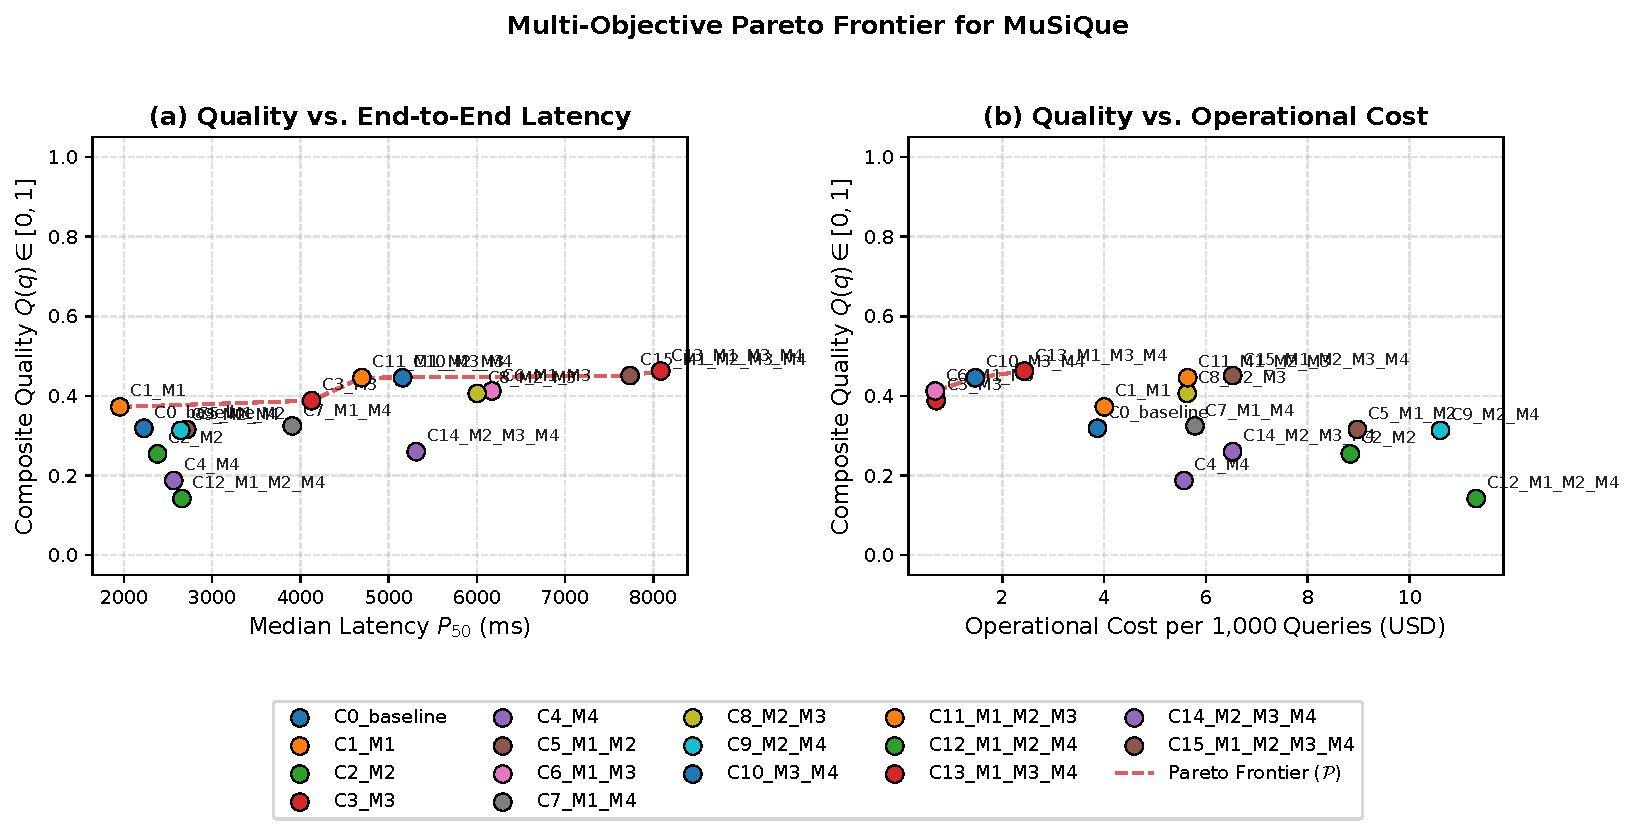
\includegraphics[width=\linewidth]{figures/musique/pareto_frontier_musique.pdf}
\caption{Empirical Pareto frontier of Composite Quality ($Q$) versus median end-to-end execution latency ($T_{\text{total}}\ P_{50}$) and operational expenditure ($\text{Cost}_{1\text{k}}$) on the academic multi-hop benchmark (MuSiQue). Solid lines delineate the non-dominated empirical Pareto frontier across configurations.}
\label{fig:pareto_frontier_musique}
\end{figure}

\subsubsection{Enterprise Production Corpus}
\label{subsubsec:pareto_enterprise}

\begin{table}[htbp]
\centering
\small
\setlength{\tabcolsep}{3.5pt}
\caption{Multi-objective Pareto efficiency and 3D non-domination trade-off metrics across 16 pipeline configurations on Enterprise Closed.}
\label{tab:pareto_enterprise}
\begin{tabular*}{\linewidth}{@{\extracolsep{\fill}} l l c r r r r c @{}}
\toprule
\textbf{Config} & \textbf{Pipeline} & \makecell{\textbf{Composite}\\\textbf{Quality $Q$}} & \makecell{\textbf{Cost / 1k}\\\scriptsize{(\$)}} & \makecell{\textbf{$T_{\text{total}} P_{50}$}\\\scriptsize{(s)}} & \textbf{QPD} & \textbf{QPS} & \makecell{\textbf{Pareto}\\\textbf{Optimal}} \\
\midrule
\multicolumn{8}{l}{\textbf{Baseline ($k=0$)}} \\
$C_{0}$ & Naive RAG Baseline & 0.7314 & \$1.339 & 1.93 & 546 & 0.23 & \textbf{Yes} \\
\midrule
\multicolumn{8}{l}{\textbf{Single-Factor Isolated ($k=1$)}} \\
$C_{1}$ & S2B & 0.5710 & \$1.464 & 1.86 & 390 & 0.11 & \textbf{Yes} \\
$C_{2}$ & SR & 0.6113 & \$6.366 & 2.38 & 96 & 0.11 & No \\
$C_{3}$ & PC & 0.6099 & \$0.640 & 3.05 & 953 & 0.12 & \textbf{Yes} \\
$C_{4}$ & MC & 0.8522 & \$1.081 & 2.25 & 788 & 0.22 & \textbf{Yes} \\
\midrule
\multicolumn{8}{l}{\textbf{Pairwise Combinations ($k=2$)}} \\
$C_{5}$ & S2B + SR & 0.6735 & \$6.435 & 3.59 & 105 & 0.06 & No \\
$C_{6}$ & S2B + PC & 0.7456 & \$0.763 & 2.11 & 977 & 0.24 & \textbf{Yes} \\
$C_{7}$ & S2B + MC & 0.5803 & \$2.014 & 3.21 & 288 & 0.03 & No \\
$C_{8}$ & SR + PC & 0.6512 & \$5.782 & 17.42 & 113 & 0.02 & No \\
$C_{9}$ & SR + MC & 0.3265 & \$7.017 & 2.98 & 47 & 0.03 & No \\
$C_{10}$ & PC + MC & 0.7474 & \$1.901 & 8.27 & 393 & 0.07 & No \\
\midrule
\multicolumn{8}{l}{\textbf{Higher-Order Triplets \& Full-Stack ($k \ge 3$)}} \\
$C_{11}$ & S2B + SR + PC & 0.6777 & \$5.714 & 2.91 & 119 & 0.12 & No \\
$C_{12}$ & S2B + SR + MC & 0.4461 & \$7.178 & 3.70 & 62 & 0.05 & No \\
$C_{13}$ & S2B + PC + MC & 0.5638 & \$0.654 & 6.80 & 862 & 0.02 & No \\
$C_{14}$ & SR + PC + MC & 0.4927 & \$7.099 & 4.05 & 69 & 0.01 & No \\
$C_{15}$ & S2B + SR + PC + MC (Full-Stack) & 0.7129 & \$5.789 & 9.35 & 123 & 0.04 & No \\
\bottomrule
\end{tabular*}
\vspace{0.5em}
\parbox{\linewidth}{\footnotesize
\textbf{Notes:} Composite Quality $Q \in [0, 1]$ represents the regularized harmonic mean across RAGAS dimensions (Equation~\ref{eq:composite_quality}, $\epsilon = 10^{-4}$). Cost reflects Google Cloud Gemini Enterprise platform pricing normalized per 1,000 queries. $T_{\text{total}} P_{50}$ represents median execution latency in seconds. Quality per Dollar ($\mathrm{QPD} = Q / \text{Cost}$) and Quality per Second ($\mathrm{QPS} = Q / T_{\text{total}}$) measure resource efficiency. Pareto optimality denotes non-domination in the 3D trade-off space $(\max Q, \min \text{Cost}, \min T_{\text{total}})$.}
\end{table}


\begin{figure}[!htbp]
\centering
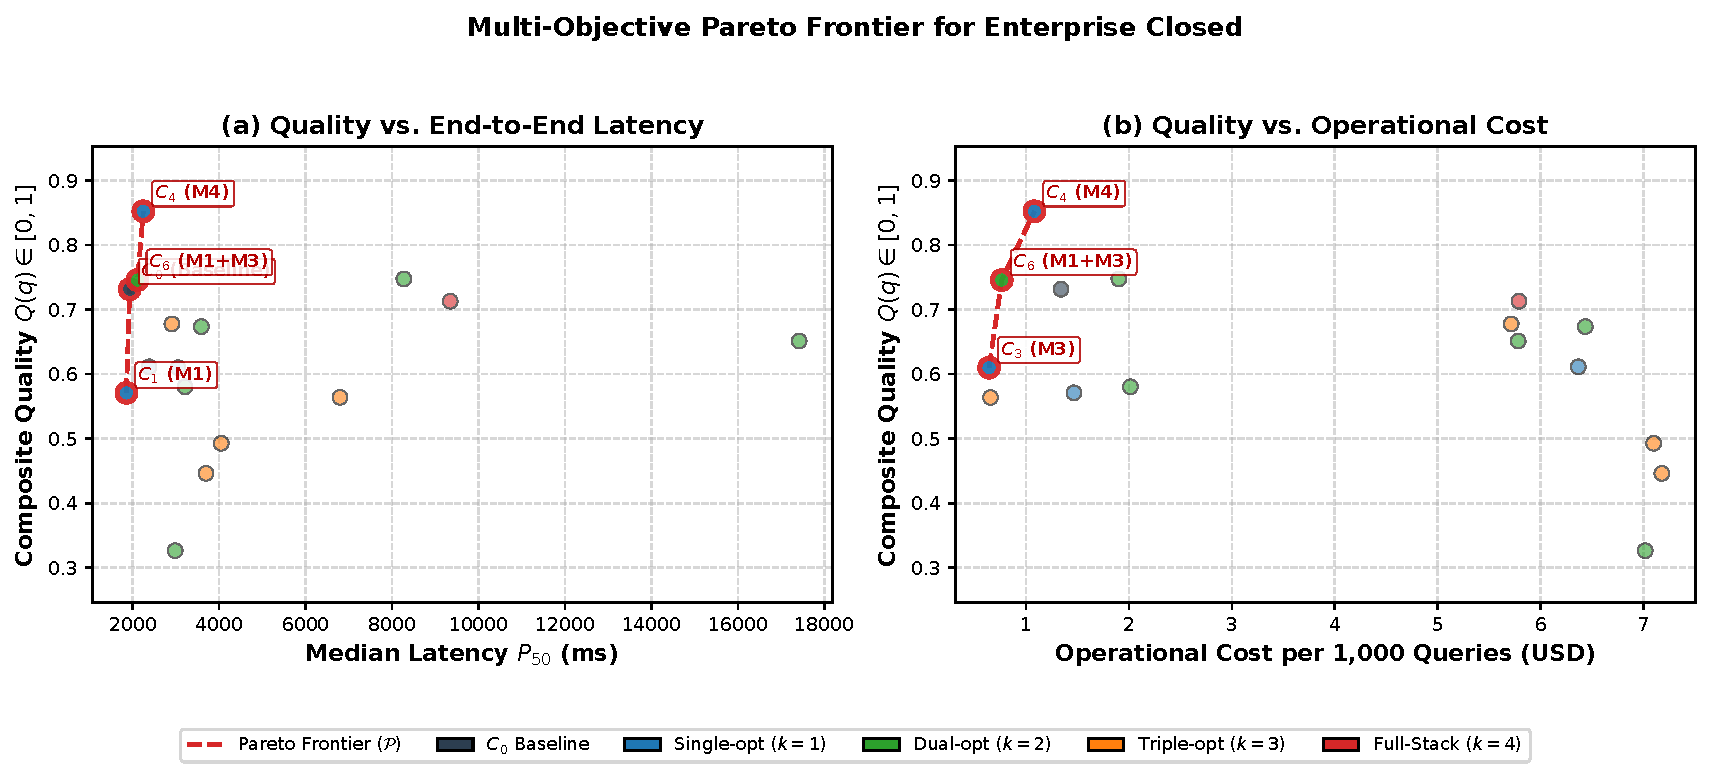
\includegraphics[width=\linewidth]{figures/enterprise_closed/pareto_frontier_enterprise_closed.pdf}
\caption{Empirical Pareto frontier of Composite Quality ($Q$) versus median end-to-end execution latency ($T_{\text{total}}\ P_{50}$) and operational expenditure ($\text{Cost}_{1\text{k}}$) on the enterprise closed benchmark corpus. Solid lines delineate the non-dominated empirical Pareto frontier across configurations.}
\label{fig:pareto_frontier_enterprise}
\end{figure}

\subsection{Executive Performance Delta Synthesis}
\label{subsec:results_delta_heatmap}

To provide a consolidated cross-dimensional view of all 15 architectural optimization treatments relative to the unoptimized naive baseline, Figure~\ref{fig:quality_delta_matrix_musique} and Figure~\ref{fig:quality_delta_matrix_enterprise} visualize relative percentage improvements (green) and regressions (red) across all four RAGAS quality dimensions, Composite Quality ($Q$), median end-to-end latency ($P_{50}$), and operational expenditure per 1,000 queries.

\begin{figure}[!htbp]
\centering
\begin{subfigure}{\linewidth}
  \centering
  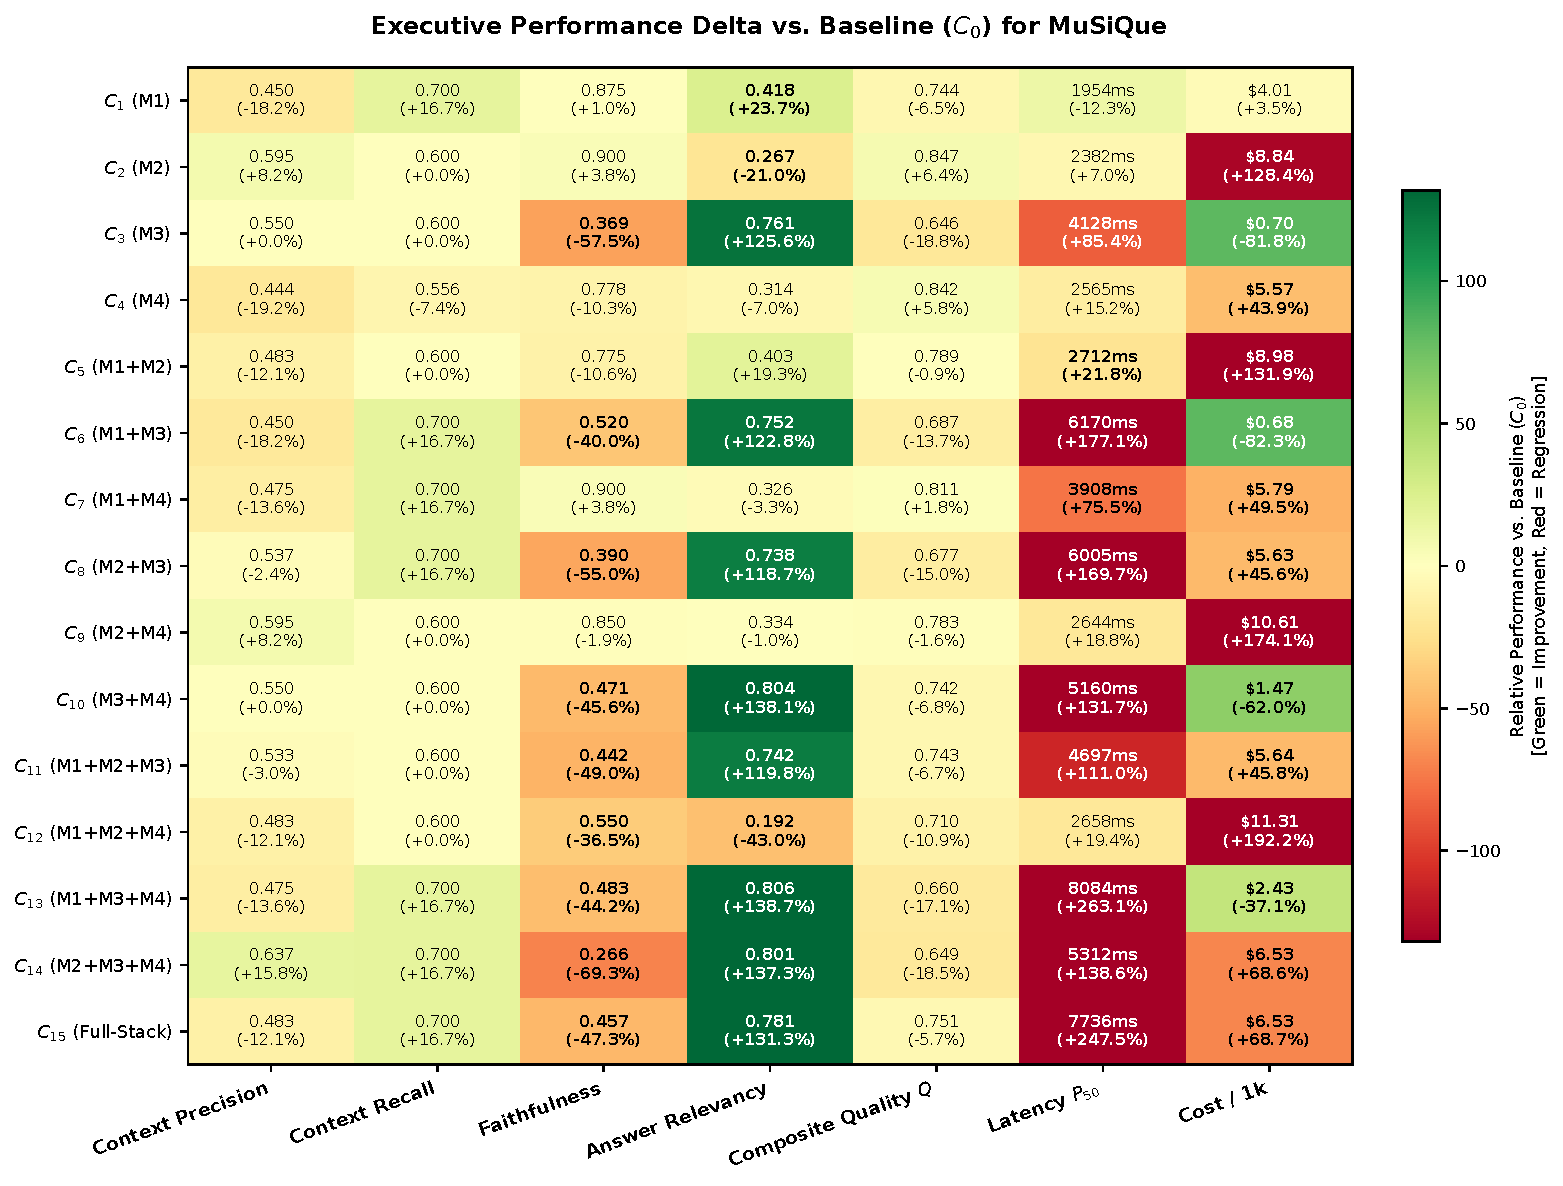
\includegraphics[width=0.78\linewidth]{figures/musique/quality_delta_matrix_musique.pdf}
  \caption{Academic multi-hop benchmark (MuSiQue)}
  \label{fig:quality_delta_matrix_musique}
\end{subfigure}
\\[1ex]
\begin{subfigure}{\linewidth}
  \centering
  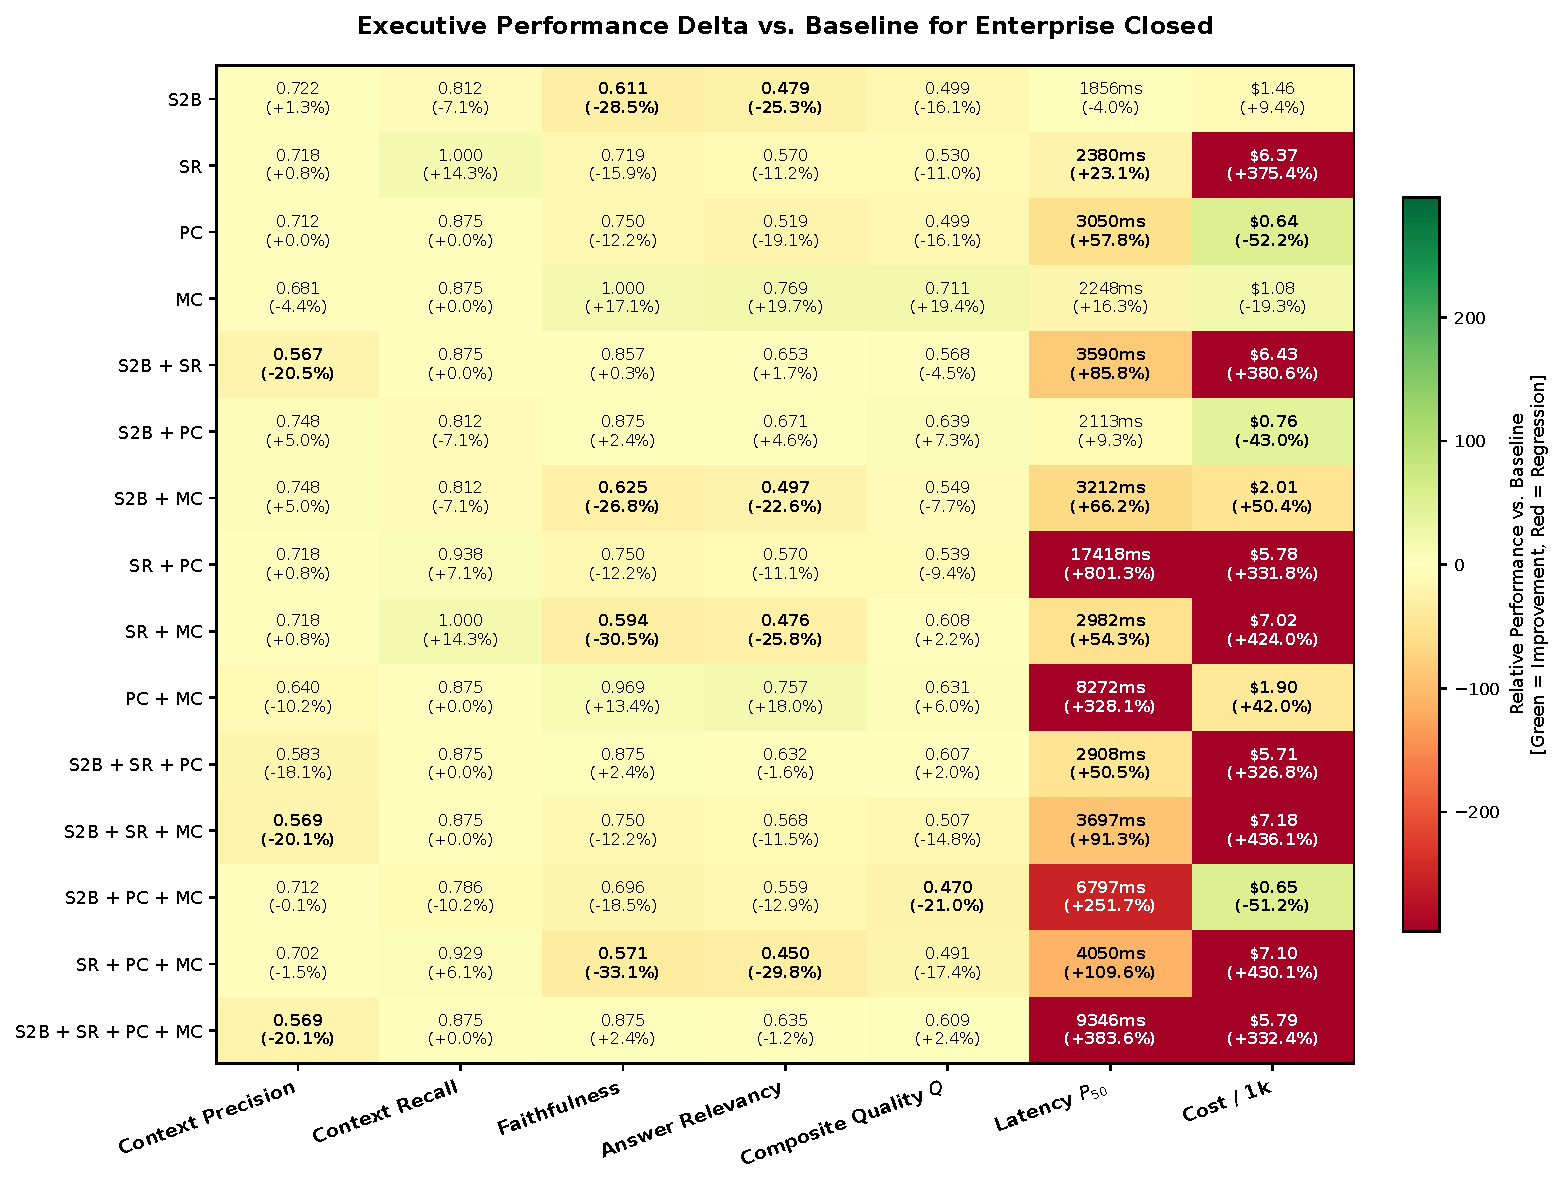
\includegraphics[width=0.78\linewidth]{figures/enterprise_closed/quality_delta_matrix_enterprise_closed.pdf}
  \caption{Enterprise closed benchmark corpus}
  \label{fig:quality_delta_matrix_enterprise}
\end{subfigure}
\caption{Executive performance delta heatmaps relative to the naive baseline on (a) MuSiQue and (b) Enterprise Closed. Cells display absolute metrics alongside relative percentage changes ($\pm\%$). Diverging color gradient highlights performance improvements (green) versus cost/latency regressions (red).}
\label{fig:quality_delta_matrix_combined}
\end{figure}


\clearpage

\section{Discussion}
\label{sec:discussion}
The idea of discussion is to bring up points that you noticed during research.
As a chapter, this is the most freeform one.
A good way to discuss the points is first to write up subtitles with clear statements and then expand on those.
Discussion points can occasionally be also in a question format or refer to a larger context beyond the thesis to bring in ideas from other papers to consider.
In case your work has limitations that you can observe, it can be a good idea to write a separate section considering those.

% =========================================================================
% DRAFT NOTES: Prompt Caching Latency Inversion in Enterprise RAG (Nordea Closed)
% =========================================================================
%
% -------------------------------------------------------------------------
% 1. EMPIIRINEN HAVAINTO (Latenssi-inversio Enterprise Closed -aineistossa, N=100)
% -------------------------------------------------------------------------
% - Vastoin intuitiota ja perusoletusta, Module M3 (Prompt Caching) ei tuo 
%   latenssihyötyjä yrityskontekstissa, vaan nostaa kokonaislatenssia:
%     * C0 Baseline:    T_total P50 = 1 407 ms | TTFT P50 = 1 135 ms
%     * C3 (M3 Prompt Caching): T_total P50 = 1 714 ms (+21.8 %) | TTFT P50 = 1 563 ms (+37.7 %)
%     * C5 (M1+M2 S2B + SR):    T_total P50 = 1 446 ms | TTFT P50 = 1 220 ms
% - C3 on merkittävästi hitaampi kuin C0 Baseline ja jopa selvästi hitaampi kuin 
%   C5 (S2B + SR), jonka odotettiin olevan raskas ylimääräisen semanttisen rerankkauksen 
%   vuoksi (rerank-vaiheen P50 = 108 ms).
%
% -------------------------------------------------------------------------
% 2. TEKNINEN JUURISYY: T_prefill ja etä-KV-cachen overhead
% -------------------------------------------------------------------------
% - Kun puretaan latenssikomponentit (context_inspector.py ja evaluoidut ajot):
%     * T_prefill C0: median = 827 ms
%     * T_prefill C3: median = 1 308 ms (+481 ms)
%     * T_stream C0:  median = 147 ms
%     * T_stream C3:  median = 105 ms
% - Itse vastaustokenien generointi (T_stream) on C3:ssa identtinen tai jopa 
%   aavistuksen nopeampi kuin C0:ssa. Koko latenssirangaistus syntyy mallin 
%   prefill-vaiheessa ennen ensimmäisen tokenin tuloa (TTFT).
% - Gemini 3.5 Flash laskee Googlen TPU-laitteistolla ~7 000 - 8 500 tokenin rinnakkaisen 
%   prefill-huomiolaskennan (attention prefill) muutamissa kymmenissä millisekunneissa.
% - Kun pyyntö käyttää Vertex AI explicit context cachingia (cachedContentName):
%     1. Vertex AI -infrastruktuuri joutuu validoimaan välimuistiviitteen ja etsimään 
%        sen hajautetusta KV-välimuistivarastosta.
%     2. Pyyntö on reititettävä tai sarjallistettu KV-tila on ladattava verkon yli 
%        juuri sille TPU-kiihdyttimelle, joka pyyntöä palvelee.
%     3. Tämä etätilan sidonta ja välimuistinhaku aiheuttaa kiinteän ~300-500 ms 
%        RPC- ja synkronointiviiveen (fixed coordination overhead).
%
% -------------------------------------------------------------------------
% 3. KONTEKSTIKOON "BREAK-EVEN" -KYNNYS
% -------------------------------------------------------------------------
% - Välimuistiin tallennettu staattinen etuliite (järjestelmäohjeet + few-shot -kirjasto, 
%   prompts/answer-generation.st) on tarkalleen 7 157 tokenia.
% - Vertex AI / Gemini Context Caching on suunniteltu massiivisille konteksteille 
%   (32k - 1M+ tokenia, esim. kirjat, koodirepot, videot). Tällöin KV-uudelleenlaskenta 
%   kestäisi sekunteja, jolloin ~300-500 ms noutoviive tuo suuren nettovoiton.
% - 7 000 tokenin kokoluokassa etävälimuistin noutaminen kestää pidempään kuin se aika, 
%   joka kuluisi tokenien puhtaaseen uudelleenlaskentaan TPU:n HBM-muistissa tyhjästä.
%   -> Yritys-RAG:ssa syntyy "latency break-even" -ongelma: konteksti on liian lyhyt 
%      latenssisäästöille, mutta ylittää palveluntarjoajan minimivälimuistikynnyksen (4 096 tok).
%
% -------------------------------------------------------------------------
% 4. KONTEKSTIVÄLIMUISTI VS. SEMANTTINEN VASTAUSVÄLIMUISTI
% -------------------------------------------------------------------------
% - M3 toteuttaa mallitason KV-kontekstivälimuistin (Gemini CachedContent), 
%   EI sovellustason semanttista vastausvälimuistia (kuten GPTCache tai Redis).
% - Vastausvälimuisti toisi osumalla 0-10 ms latenssin, mutta kontekstivälimuistissa 
%   LLM joutuu aina suorittamaan uuden päättelyn ja generoinnin dynaamisesti 
%   noudetuille yritysdokumenteille.
%
% -------------------------------------------------------------------------
% 5. DIPLOMITYÖN TULOS & PARETO-ANALYYSI (RQ1 vs. RQ2)
% -------------------------------------------------------------------------
% - Prompt Caching ei toimi yritystason RAG:ssa latenssinoptimoijana, vaan puhtaana 
%   kustannusoptimointina:
%     * Latenssi (RQ1): T_total nousee +21.8 % (1 407 ms -> 1 714 ms).
%     * Kustannus (RQ2): Ajokustannus putoaa -70.7 % ($13.58 -> $3.98 / 1k kyselyä; 
%       yhdessä M4-reitityksen kanssa jopa $2.54 / 1k eli -81.3 %).
% - Laatu (RQ3): F1 säilyy identtisenä (C0: 59.4 % vs. C3: 58.8 %).
% - Johtopäätös: Järjestelmäarkkitehdin on tehtävä tietoinen Pareto-valinta: 
%   ollaanko valmiita maksamaan ~300 ms lisälatenssia käyttäjälle vastineena yli 
%   70 % operatiivisesta pilvikustannussäästöstä.
%
% =========================================================================
% DRAFT NOTES 1B: Prompt Caching Häntälatenssin Sulakkeena (Circuit-Breaker)
% =========================================================================
% - Vaikka PC nostaa mediaanilatenssia, MuSiQuessa se toimii kriittisenä 
%   P95-häntälatenssin leikkurina monivaiheisissa ketjuissa:
%     * S2B + SR (C5):    P95 = 7 771 ms -> S2B + SR + PC (C11):    P95 = 2 202 ms (-71.7 %)
%     * S2B + MC (C7):    P95 = 14 154 ms -> S2B + PC + MC (C13):   P95 = 4 644 ms (-67.2 %)
%     * S2B + SR + MC (C12): P95 = 30 883 ms -> S2B + SR + PC + MC (C15): P95 = 4 306 ms (-86.1 %)
%     * S2B + PC (C6):    P50 = 1 250 ms (-8.0 %, p < 0.001) ja P95 = 1 745 ms (baseline: 3 397 ms)
% - JSONL-raakadata paljastaa: Ilman välimuistia monimutkaiset ketjut kärsivät satunnaisista 
%   20-90 s TPU-muistinvaraus- ja jonotuspiikeistä ruuhka-aikoina (esim. C12 kyselyssä 
%   3hop1__135793_87694_64412: T_prefill = 89.7 s).
% - Cachen käyttö eliminoi nämä ääripiikit, koska 7 157 tokenin esilaskettu tila on jo 
%   valmiiksi kiinnitetty TPU:n muistiin. PC toimii siis SLA-sulakkeena (Circuit-Breaker).
%
% =========================================================================
% DRAFT NOTES 2: Frontier-mallin (Gemini 3.1 Pro) Over-Refusal Paradox (RQ3 / M4)
% =========================================================================
% - Reititysjakautuma:
%     * MuSiQue: Pro-dominantti (77 % Pro, 21 % Flash, 2 % Lite; 3/4-hop 100 % Pro).
%     * Enterprise Closed: Lite/Flash-dominantti (49 % Lite, 38 % Flash, 13 % Pro; 
%       1-hop 97.5 % Lite, 2-hop 67.5 % Flash / 30 % Pro).
% - Paradoksi MuSiQuessa: Frontier-malli Gemini 3.1 Pro kieltäytyy vastaamasta 
%   vastattaviin kysymyksiin huomattavasti herkemmin kuin Gemini 3.5 Flash:
%     * C0 Baseline (Flash): FRR = 42.5 %
%     * C4 MC (Pro-dominantti): FRR = 63.9 % (Pron oma FRR vastattavissa = 63.9 %)
%     * C14 SR+PC+MC: FRR = 78.3 % Prolla (koko putken FRR = 68.8 %)
% - Juurisyy JSONL-datassa (Ehdollinen Context Recall -analyysi):
%     * Kun haettu konteksti on osittainen (CR < 1.0, eli 1 välihyppy puuttuu top-5:stä):
%       Pro kieltäytyy 87.0 % - 96.8 % ajasta, kun taas Flash kieltäytyy vain 50.0 % - 68.6 % 
%       ja kykenee päättelemään puuttuvan askeleen.
%     * Täydelläkin kontekstilla (CR = 1.0) Pro kieltäytyy 42.3 % - 58.6 % ajasta monimutkaisissa 
%       monihyppytehtävissä tulkiten synteesin epävarmaksi (Flash kieltäytyy vain 0 - 22 %).
% - Johtopäätös: Pron tiukka RLHF- ja grounding-ohjeistus tekee siitä tuotantoon turvallisen 
%   (100 % OOD Refusal Accuracy), mutta se rankaisee monihyppyhaun osittaista osumatarkkuutta.
%
% =========================================================================
% DRAFT NOTES 3: Synergia-bifurkaatio: SR + MC (C9) romahdus vs. S2B + MC (C7) menestys
% =========================================================================
% - Enterprise Closedissa havaitaan jyrkkä laatuero:
%     * S2B + MC (C7):  Q = 0.6587 (toiseksi paras), Faith = 0.858, FRR = 11.2 %
%     * SR + MC (C9):   Q = 0.5418 (koko testin huonoin, -12.7 %), Faith = 0.780, FRR = 17.5 %
%     * Huom: C9:llä on silti koko testin KORKEIN Context Precision (0.683 vs. C7:n 0.661)!
% - Juurisyy JSONL-datasta (Kyselyt 1hop__nordea_0030, 2hop__nordea_0009, 0019, 0020, 0040):
%     * Re-ranker ilman S2B-laajennusta karsii pois reunaehtojen ja 2-hypyn taustakappaleet 
%       (kontekstin pituus putoaa 4.5k merkkiin vs. C7:n 8.1k merkkiin).
%     * Flash-Lite ei kykene rekonstruoimaan puuttuvia ehtoja kapeista paloista: se kieltäytyy 
%       tai hallusinoi ehtoja (Faithfulness putoaa Litellä 0.906 -> 0.849, esim. kysely 0040: Faith = 0.50).
%     * Pro kieltäytyy herkästi puutteellisella kontekstilla (Pron FRR C9:ssä peräti 50.0 %!).
%     * C7:ssä S2B:n 1 024 tokenin vanhempidokumentti toimii suojakilpenä: Litellä FRR on 
%       vain 2.4 % ja Faithfulness 0.906. S2B suojaa kevyitä ja tiukkoja malleja pirstaloitumiselta.
%
% =========================================================================
% DRAFT NOTES 4: Hakukohinan Kynnysarvo (Retrieval Noise Threshold) & Korpusten Inversio
% =========================================================================
% - Suljetussa korpuksessa (Enterprise Closed, 20 kandidaattia / kysely, 1 701 palaa):
%     * C1 S2B pärjää yksin erinomaisesti (Q = 0.6449 ns).
%     * Re-rankingin lisääminen (C5 S2B + SR) LASKEE laatua (Q = 0.5813 ns), koska puhdas 
%       kanta ei tarvitse karsintaa ja re-ranker rikkoo peräkkäisten lapsipalojen koheesion.
% - Avoimessa raakakorpuksessa (Enterprise Raw, 2 420 uniikkia palaa, PDF-ehdot ja web):
%     * Baseline C0 romahtaa (Q = 0.5022, 2-hop FRR hyppää 12.5 % -> 27.5 %).
%     * Re-ranking toimii välttämättömänä kohinasuodattimena (Noise Gate), joka siivoaa distraktorit 
%       ennen S2B-laajennusta:
%         - S2B + SR (C5):    Q = 0.6433** (p_adj = 0.0077, +28.1 % parannus baselineen)
%         - S2B + SR + PC (C11): Q = 0.6466** (p_adj = 0.0029, +28.8 % parannus)
%         - S2B + SR + MC (C12): Q = 0.6162*  (p_adj = 0.0470, +22.7 % parannus)
%         - Context Precision paranee tilastollisesti merkitsevästi (p_adj < 0.05) peräti 7 S2B-putkessa.
%         - 2-hop FRR putoaa 27.5 %:sta 7.5 %:iin!
% - Johtopäätös: Re-ranking tuo tilastollisesti vahvistetun hyödyn vasta, kun hakukohina 
%   ylittää kriittisen kynnysarvon. Kuratoidussa kannassa se on redundanssi.
%
% =========================================================================
% DRAFT NOTES 5: Harmonisen Keskiarvon Q (eps = 10^-4) "Heikoimman Lenkin Rangaistus"
% =========================================================================
% - Säännöllistetyn harmonisen keskiarvon kaava (Eq. 4.25):
%     * Jos YKSIKIN neljästä metriikasta (CP, CR, Faith, AR) on 0.0:
%       nimittäjään tulee 1/10^-4 = 10 000, jolloin Q(q) romahtaa välittömästi arvoon <= 0.0004.
% - Empiirinen todiste: MuSiQuessa 68.8 % - 77.5 % vastattavista kyselyistä sisältää vähintään 
%   yhden nollametristen (useimmiten FRR:n aiheuttama Faith=0, AR=0 tai noudon CR=0).
% - Tilastollinen seuraus: Koska yli puolet otoksesta on nollassa, mediaani-Q naulautuu arvoon 
%   0.0002 kaikilla putkilla, ja parittainen mediaaniero muuttuu muotoon mu_delta = 0.0000.
% - Tämä nollaa parametrittoman Wilcoxon-testin tilastollisen voiman (sidokset / ties).
% - Metodologinen opetus: Harmoninen Q on ankara teollinen luotettavuusmittari (penalizes single-point-of-failure), 
%   mutta tilastolliseen hypoteesitestaukseen se vaatii suuren otoskoon tai jatkuvamman metriikan.
%
% =========================================================================
% DRAFT NOTES 6: Poikkileikkaavat Havainnot (PC Attention Anchoring & S2B Latenssi)
% =========================================================================
% - PC:n huomion ankkurointivaikutus (Attention Anchoring):
%     * C6 (S2B + PC) saavuttaa korkeamman Faithfulnessin (0.886) kuin C1 S2B (0.863).
%     * Staattisen kehotteen ja CoT-esimerkkien jäädyttäminen KV-cacheen ankkuroi huomion, 
%       estäen tarkkaavaisuuden hajoamista (attention dilution / drift) pitkissä 1 024 tokenin ikkunoissa.
% - Small-to-Bigin negatiivinen latenssidelta yritysaineistoissa (-4.3 % Closed, -2.4 % Raw):
%     * PostgreSQL:n parent-laajennus vie vain 1-2 ms (T_expand).
%     * Kompaktimpi 128 tokenin lapsi-indeksi leikkaa noudon P95-häntälatenssin puoleen (674 -> 317 ms).
%     * Eheä parent-konteksti nopeuttaa LLM:n striimausta (T_stream P50: 147 -> 131.5 ms), koska 
%       malli vastaa varmemmin ilman epävarmuuden kiertelyä.
%



\clearpage

\section{Conclusion}
\label{sec:conclusion}
% Template notes:
% The idea of the conclusion is the opposite of the introduction.
% Here we literally bring the reader out of the topic, not in.
% A good way to write conclusion is to start by reminding the reader of your research question(s) and then state how your work addressed them.
% To finish your conclusion, consider open research questions (this can be a list for example).

% =========================================================================
% SUOSITELTU KAPPALERAKENNE LUKUUN 7 (Ilman \subsection-otsikoita, ~1.5-2 s.)
% =========================================================================
%
% -------------------------------------------------------------------------
% 1. KOKOAVA AVAUSKAPPALE (1 kappale)
% -------------------------------------------------------------------------
% - Muistuttaa lukijaa työn päätavoitteesta ja kontribuutiosta: neljän
%   modulaarisen RAG-optimoinnin (Small-to-Big Retrieval, Semantic Re-ranking,
%   Prompt Caching ja Model Cascading) sekä niiden 16 täysfaktoriaalisen
%   yhdistelmän (C0...C15) empiirinen arviointi tuotantotason Java / Spring AI
%   -arkkitehtuurissa akateemisen monihyppyaineiston (MuSiQue) ja aidon
%   yritystietokannan (Enterprise Closed & Raw) yli.
%
% -------------------------------------------------------------------------
% 2. VASTAUKSET TUTKIMUSKYSYMYKSIIN RQ1–RQ4 (1–2 kappaletta tai \textbf{RQ1...})
% -------------------------------------------------------------------------
% - Tiivistää suorat, kvantitatiiviset vastaukset Johdannon tutkimuskysymyksiin
%   (Table 1, 01_introduction.tex) 2–3 virkkeellä per kysymys:
%     * RQ1 (Latency): Modulaariset optimoinnit harvoin alentavat mediaanilatenssia
%       (poikkeuksena S2B + PC MuSiQuessa -8.0 % ja S2B:n kevyt etu yritysdatassa).
%       PC tuo etä-KV-haun vuoksi ~300 ms mediaanilisän, mutta toimii kriittisenä
%       P95-häntälatenssin sulakkeena (circuit-breaker, jopa -86 %). MC kasvattaa
%       latenssia etenkin frontier-mallille reititettäessä.
%     * RQ2 (Cost): Prompt Caching on tehokkain yksittäinen kustannusvipu
%       (-70.7 % ... -80.0 %). Yrityskorpuksessa MC kääntää kustannukset laskuun
%       (-34.2 %), ja yhdistelmä PC + MC saavuttaa jopa 81.3 % säästön ($2.54 / 1k)
%       sekä kompensoi täysin monivaiheisen haun (S2B + SR) API-kustannukset.
%     * RQ3 (Quality): Suljetuissa korpuksissa naiivi baseline on vahva, eikä
%       yksittäinen optimointi ylitä sitä tilastollisesti merkitsevästi; S2B + PC
%       saavuttaa korkeimman kokonaislaadun (Q = 0.6711) ja 100 % OOD-tarkkuuden.
%       Suodattamattomassa yrityskannassa (Raw) S2B + SR -yhdistelmä tuottaa
%       tilastollisesti merkitsevän (+28.1 % ... +28.8 %) laatuparannuksen.
%     * RQ4 (Interaction & Pareto Equilibrium): Kolme arkkitehtuuria (Baseline,
%       PC ja S2B + PC) pysyy Pareto-optimaalisina kaikilla korpuksilla. Moduulien
%       välillä esiintyy vahva synergia-bifurkaatio: S2B suojaa MC:tä kontekstin
%       pirstaloitumiselta (S2B + MC), kun taas pelkkä re-ranking yhdistettynä
%       reititykseen (SR + MC) heikentää synteesin luotettavuutta.
%
% -------------------------------------------------------------------------
% 3. JATKOTUTKIMUSAIHEET / FUTURE WORK & LOPETUS (1–2 kappaletta)
% -------------------------------------------------------------------------
% - Nostaa esiin keskeiset jatkotutkimussuunnat:
%     1. Iteratiivinen ja agenttipohjainen monihyppyhaku (multi-step / agentic RAG)
%        yksivaiheisen (single-shot) haun 3–4 hypyn laatukaton murtamiseksi.
%     2. Kaksitasoinen välimuistiarkkitehtuuri: mallitason KV-kontekstivälimuistin
%        (Prompt Caching) yhdistäminen sovellustason semanttiseen vastausvälimuistiin
%        sekä kustannusten että TTFT-latenssin minimoimiseksi.
%     3. Monikielinen yritys-RAG (cross-lingual retrieval & synthesis, esim.
%        pohjoismaiset pankkiaineistot FI/SV/DA/NO/EN) ja dynaaminen palastelu.
%     4. Monipilvi- ja avoimen lähdekoodin malliperheiden vertailu reitityksessä.
% - Kokoava lopetusvirke: tasapaino operatiivisen tehokkuuden ja vastausten
%   luotettavuuden välillä yritystason tekoälyjärjestelmissä.



\clearpage
\bibliographystyle{unsrtnat}
\bibliography{references/ai}
